\documentclass{article}
\usepackage[margin=1in]{geometry}
\usepackage[nodisplayskipstretch]{setspace}
\usepackage{amsmath, nccmath, bm}
\usepackage{amssymb}
\usepackage{enumitem}
\usepackage{graphicx}
\usepackage{float}
\usepackage{listings}
\usepackage{hyperref}
\usepackage[svgnames]{xcolor}
\usepackage{indentfirst}
%\usepackage{chngcntr}
%\counterwithin{table}{section}
\graphicspath{
{./images}
{./images/nand}
{./images/nand/delay}
{./images/nand/design}
{./images/nand/noise_analysis}
{./images/nand/power}
{./images/nand/vtc}
{./images/nor}
{./images/nor/delay}
{./images/nor/design}
{./images/nor/noise_analysis}
{./images/nor/power}
{./images/nor/vtc}
{./images/nmos}
{./images/pmos}}

%\hypersetup{
%    colorlinks=true,
%    linkcolor=black,
%    filecolor=black,      
%    urlcolor=blue
%    }

\newcommand{\zerodisplayskip}{
	\setlength{\abovedisplayskip}{0pt}%
	\setlength{\belowdisplayskip}{0pt}%
	\setlength{\abovedisplayshortskip}{0pt}%
	\setlength{\belowdisplayshortskip}{0pt}%
	\setlength{\mathindent}{0pt}}
	
\definecolor{vgreen}{RGB}{104,180,104}
\definecolor{vblue}{RGB}{49,49,255}
\definecolor{vorange}{RGB}{255,143,102}

\lstdefinestyle{verilog-style}
{
    language=Verilog,
    basicstyle=\small\ttfamily,
    keywordstyle=\color{vblue},
    identifierstyle=\color{black},
    commentstyle=\color{vgreen},
    numbers=left,
    numberstyle=\tiny\color{black},
    numbersep=10pt,
    tabsize=8,
    moredelim=*[s][\colorIndex]{[}{]},
    literate=*{:}{:}1
}

\lstset{style={verilog-style},showstringspaces=false}

\makeatletter
\newcommand*\@lbracket{[}
\newcommand*\@rbracket{]}
\newcommand*\@colon{:}
\newcommand*\colorIndex{%
    \edef\@temp{\the\lst@token}%
    \ifx\@temp\@lbracket \color{black}%
    \else\ifx\@temp\@rbracket \color{black}%
    \else\ifx\@temp\@colon \color{black}%
    \else \color{vorange}%
    \fi\fi\fi
}
\makeatother

\newcommand{\code}[1]{%
	\colorbox{Gainsboro}{\texttt{#1}}%
}

\title{Lab 1}
\author{Owen Sowatzke}
\date{March 19, 2025}

\begin{document}

	% \offinterlineskip
	% \setlength{\lineskip}{12pt}
	% \zerodisplayskip
	\maketitle
	
	\section{Introduction}
	
	In this lab, we use xschem to draw and simulate NAND and NOR gates built using SkyWater 130nm technology. Following the procedure described for the inverter, we determine the voltage transfer characteristics, noise margins, delay, and power of each gate. For comparison, we also use the equations presented in class to theoretically compute these parameters. The equations presented in class are based on a first-order MOSFET model. To determine the parameters in these model, we fit the first-order MOSFET equations to measured the IV characteristics of the NMOS and PMOS gates. This work is included for reference in Appendices \ref{appendix::nmos_iv_characteristics} and \ref{appendix::pmos_iv_characteristics}.
	
	\section{NAND Gate}
	
	In this section, we analyze the NAND gate built using SkyWater 130nm technology. We start by drawing a NAND gate and its corresponding symbol in xschem. Next, using ngspice, we analyze the voltage transfer characteristics of the gate, determining the switching threshold, $V_M$, and the noise margins. Then, using transient analysis, we measure the delay of the gate and its power consumption. For each value that we measure, we also compute a theoretical-equivalent using the equations provided in class.
	
	\subsection{Design}
	
	The NAND gate pull-down circuit is composed of two NMOS transistors in series. The pull-up circuit is the complement of the pull-down circuit and is composed of two parallel PMOS transistors. To determine the optimum sizing of the transistors in each network, we consider the equivalent resistance of each network. Compared to an inverter, the equivalent resistance of the pull-down network is doubled because the NMOS transistors are laid out in series. For the pull-up network, we consider the worst (slowest) case, in which only one PMOS transistor turns on. In this case, the pull-up network resistance is equivalent to that of an inverter. To account for differences in resistance, we need to double the width of the NMOS transistors, which halves their resistance. 
	
	For an inverter, we need to make the width of the PMOS transistor twice as large as the width of the NMOS transistor because the mobility of holes is lower than the mobility of electrons. After accounting for differences in resistances, we find that the NMOS and PMOS widths should be the same in an NAND gate. To match the behavior of the inverter with a NMOS width of 1 and a PMOS width of 2, we make the NMOS width 2 and the PMOS width 2. The NAND gate circuit with these transistor widths is shown in Figure \ref{fig::nand_schematic}.
	
	\begin{figure}[H]
		\centerline{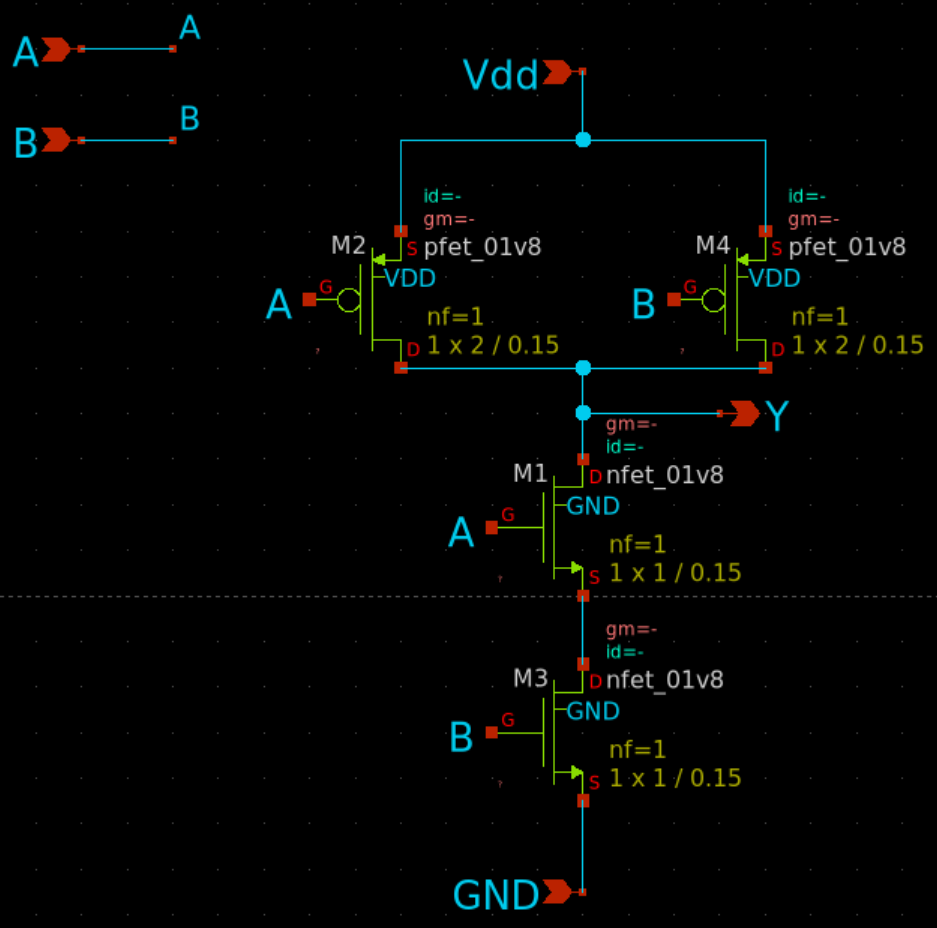
\includegraphics[width=0.4\textwidth]{nand_schematic.png}}
		\caption{NAND Circuit Schematic}
		\label{fig::nand_schematic}
	\end{figure}

	\noindent We also create a circuit symbol for the NAND gate, to allow reuse in other schematics. This circuit symbol is shown in Figure \ref{fig::nand_symbol}.
	
	\begin{figure}[H]
		\centerline{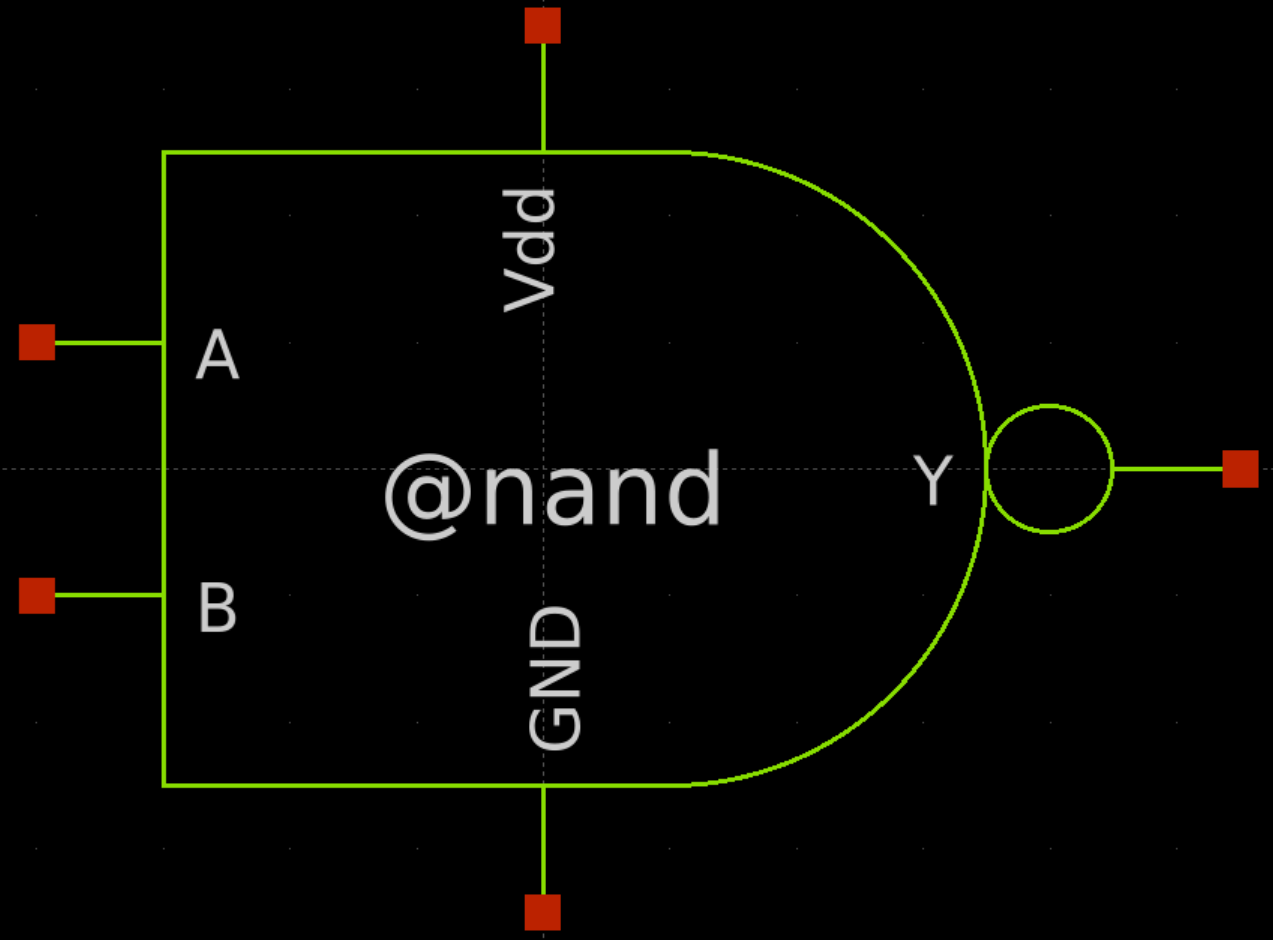
\includegraphics[width=0.4\textwidth]{nand_symbol.png}}
		\caption{NAND Circuit Symbol}
		\label{fig::nand_symbol}
	\end{figure}
	
	\subsection{Voltage Transfer Characteristics}
	
	In this section, we analyze the voltage transfer characteristics (VTC) of our NAND gate. For this analysis, we analyze the VTC for all combinations of inputs that lead to an output logic level change. When generating the VTC in ngspice, we consider consider only one set of transitions because the steady state output voltages are the same regardless of which direction we sweep. As such, we analyze the input voltages that result in high-to-low transitions. These voltages are dictated in Table \ref{table::nand_gate_high_to_low_transitions}.
	
	\begin{table}[H]
	\begin{center}
	\caption{Inputs that Create High to Low Transition for NAND Gate}
	\label{table::nand_gate_high_to_low_transitions}
	\begin{tabular}{| c | c |}
		\hline
		\texttt{a} & \texttt{b} \\
		\hline	
		$0 \rightarrow 1$ & $1$\\
		\hline	
		$1$ & $0 \rightarrow 1$\\
		\hline	
		$0 \rightarrow 1$ & $0 \rightarrow 1$\\
		\hline
	\end{tabular}
	\end{center}
	\end{table}
	
	\noindent The test circuit we use to generate the VTC for the first entry in the table is given in Figure \ref{fig::nand_vtc_test_sweep_va}.
	
	\begin{figure}[H]
		\centerline{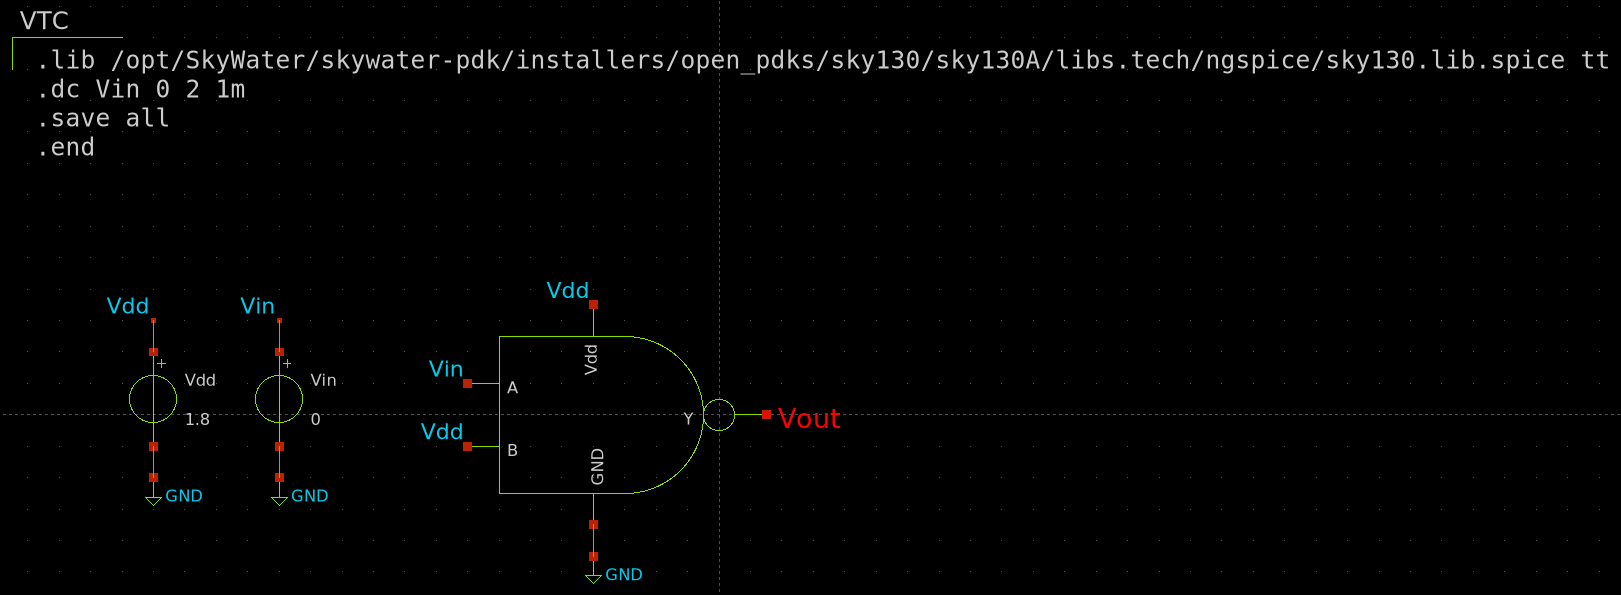
\includegraphics[width=0.8\textwidth]{nand_vtc_test_sweep_va.png}}
		\caption{NAND VTC Test Circuit for Variations of \texttt{a} with \texttt{b=1}}
		\label{fig::nand_vtc_test_sweep_va}
	\end{figure}	
	
	\noindent Using this test circuit, we perform DC analysis to generate the VTC and find $V_M$, which is the voltage at which $V_{in} = V_{out}$. The results of this analysis are shown in Figure \ref{fig::nand_vtc_sweep_va}.
	
	\begin{figure}[H]
		\centerline{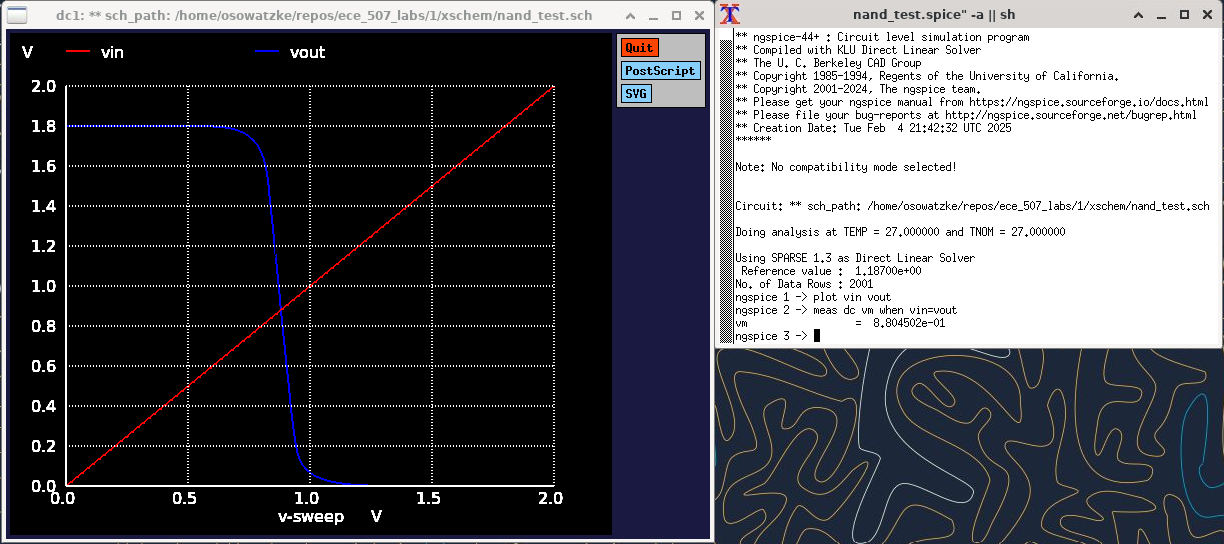
\includegraphics[width=0.8\textwidth]{nand_vtc_sweep_va.png}}
		\caption{NAND VTC Results for Variations of \texttt{a} with \texttt{b=1}}
		\label{fig::nand_vtc_sweep_va}
	\end{figure}
	
	Examining the results, we find that $V_M = 0.8257\ \text{V}$. With slight modifications to our test circuit, we can find $V_M$ for the other sets inputs listed in Table \ref{table::nand_gate_high_to_low_transitions}. These results are included in Table \ref{table::nand_gate_vm}.
	
	\begin{table}[H]
	\begin{center}
	\caption{\texttt{Vm} for Each Set of Inputs That Result in an Output Logic Level Change}
	\label{table::nand_gate_vm}
	\begin{tabular}{| c | c | c |}
		\hline
		\texttt{a} & \texttt{b} & \texttt{Vm}\\
		\hline	
		$0 \rightarrow 1$ & $1$ & $0.8257 \text{V}$\\
		\hline	
		$1$ & $0 \rightarrow 1$ & $0.8195 \text{V}$\\
		\hline	
		$0 \rightarrow 1$ & $0 \rightarrow 1$ & $0.9108 \text{V}$\\
		\hline
	\end{tabular}
	\end{center}
	\end{table}
	
	\noindent Reviewing our captured results, we see that $V_M$ is dependent on the gate inputs. $V_M$ is the largest when both gates switch at the same time. This makes sense because our pull-up network is strongest in this case, causing $V_M$ to shift to the right.
	
	We can solve the IV equations to find $V_M$ analytically. However, that can get complicated, especially for gates more complex than an inverter. When both inputs switch at the same time, we can instead use an equivalent inverter model described in \cite{cmos_vlsi_design, equivalent_inverter, inverter_dc_analysis}. In the equivalent inverter model, we treat the gate as an inverter and scale the NMOS and PMOS transistors to reflect the series and parallel transistors. For parallel connections, the equivalent resistance will be halved, and for series connections, the equivalent resistance will be doubled. For an NAND gate, this is equivalent to doubling the PMOS width and halving NMOS width.
	
	In an inverter (assuming velocity saturation), we can solve for $V_M$ as follows:
	
	\begin{equation}
		\label{eq::vm}
		V_{M} = \frac{\left(V_{T_n} + \frac{V_{DSAT_n}}{2}\right) + r\left(V_{DD} + V_{T_p} + \frac{V_{DSAT_p}}{2}\right)}{1 + r}
	\end{equation}
	
	\noindent where:
	
	\begin{equation}
		\label{eq::beta_ratio}
		r = \frac{\beta_pV_{DSAT_p}}{\beta_nV_{DSAT_n}} = \frac{k_pW_pV_{DSAT_p}}{k_nW_nV_{DSAT_n}}
	\end{equation}
	
	\noindent In Equation \ref{eq::beta_ratio}, we use the transistor widths of the equivalent inverter. Then, we substitute parameters from Appendix \ref{appendix::nmos_iv_characteristics} and \ref{appendix::pmos_iv_characteristics}, to find $V_M$. Doing so, we find that $V_M \approx 0.8404\ \text{V}$. Note that this estimate is off for a few reasons. First, Equation \ref{eq::vm} assumes that both devices are operating in the velocity saturation state which is not the case here ($|V_{gs} - V_t| < |V_{DSAT}|$ for both the NMOS and PMOS transistors). Secondly, the first order model presented in class does not do a good job of representing the current in the transition between linear and velocity saturation regions, where $V_M$ is unfortunately defined. 
	
	\subsection{Noise Analysis}
	\label{section::nand_noise_analysis}
	
	Using the test circuit shown in Figure \ref{fig::nand_vtc_test_sweep_va}, we can also measure the noise margins, which are defined follows:
	
	\begin{equation}
		NM_H = V_{OH} - V_{IH}
		\label{eq::noise_margin_high}
	\end{equation}
	
	\begin{equation}
		NM_L = V_{IL} - V_{OL}
		\label{eq::noise_margin_low}
	\end{equation}
	
	In the above formulas, $V_{IH}$ and $V_{IL}$ are defined as the unity points of the gain function, where the gain function is defined as the derivative of the VTC. For the case in which we vary \texttt{a} with \texttt{b=1}, we can identify the unity gain points and solve for the noise margins.
	
	\begin{figure}[H]
		\centerline{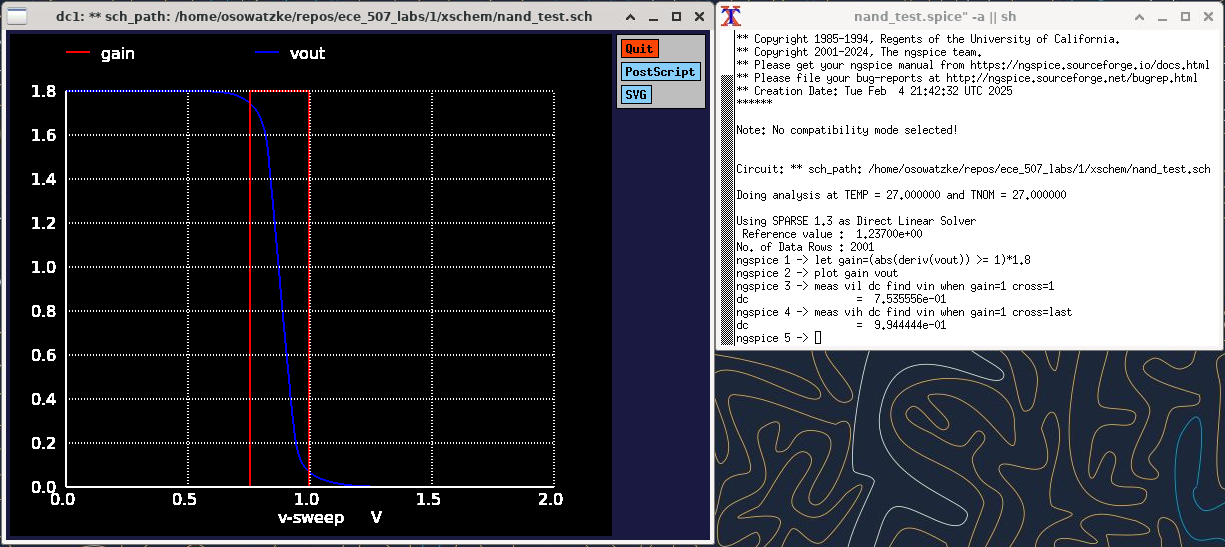
\includegraphics[width=0.8\textwidth]{nand_noise_analysis_sweep_va.png}}
		\caption{Measuring Noise Margins for the NAND Gate when \texttt{a} is Varied and \texttt{b=1}}	\label{fig::nand_noise_analysis_sweep_va}
	\end{figure}
	
	Examining the outputs shown in Figure \ref{fig::nand_noise_analysis_sweep_va}, we find that $V_{IL} = 0.6926\ \text{V}$ and $V_{IH} = 0.9264\ \text{V}$. This implies that $NM_{H} = 1.8\ \text{V} - 0.9264 \text{V} = 0.8736 \text{V}$ and $NM_{L} = 0.6926 \text{V} - 0 \text{V} = 0.6926 \text{V}$. With slight modifications to the test circuit, we can also measure the noise margins for the additional sets of inputs listed in Table \ref{table::nand_gate_high_to_low_transitions}. Our results for this analysis are listed in Table \ref{table::nand_gate_noise_analysis}.
	
	\begin{table}[H]
	\begin{center}
	\caption{Noise Margins for Each Set of Inputs That Result in an Output Logic Level Change}
	\label{table::nand_gate_noise_analysis}
	\begin{tabular}{| c | c | c | c | c | c |}
		\hline
		\texttt{a} & \texttt{b} & \texttt{Vih} & \texttt{Vil} & \texttt{Nmh} & \texttt{Nml} \\
		\hline	
		$0 \rightarrow 1$ & $1$ & $0.9264 \text{V}$ & $0.6926 \text{V}$ & $0.8736 \text{V}$ & $0.6926 \text{V}$\\
		\hline	
		$1$ & $0 \rightarrow 1$ & $0.9184 \text{V}$ & $0.7116 \text{V}$ & $0.8816 \text{V}$ & $0.7116 \text{V}$\\
		\hline	
		$0 \rightarrow 1$ & $0 \rightarrow 1$ & $1.0224 \text{V}$ & $0.8046 \text{V}$ & $0.7776 \text{V}$ & $0.7776 \text{V}$\\
		\hline
	\end{tabular}
	\end{center}
	\end{table}
	
	For comparison, we also compute the noise margins using the equations presented in class. For this analysis, we consider the case where \texttt{a} and \texttt{b} vary together. This allows us to analyze the circuit with an equivalent inverter model. For our theoretical analysis, we also consider Figure \ref{fig::noise_margins_theory}, which is provided in \cite{rabaey_2003_digital}.
	
	\begin{figure}[H]
		\centerline{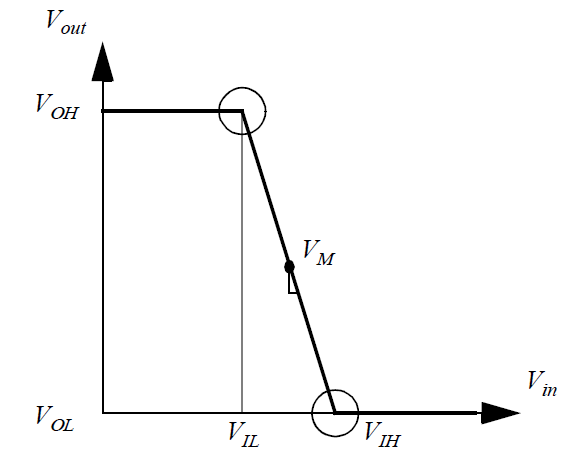
\includegraphics[width=0.4\textwidth]{noise_margins_theory.png}}
		\caption{Theoretical Noise Margins Analysis}
		\label{fig::noise_margins_theory}
	\end{figure}
	
	\noindent From the graph, we see that we can define $V_{IL}$ and $V_{IH}$ as follows:
	
	\begin{equation}
		\label{eq::vih_theory}
		V_{IH} = V_{M} - \frac{V_M}{g}
	\end{equation}
	
	\begin{equation}
		\label{eq::vil_theory}
		V_{IL} = V_{M} + \frac{V_{DD} - V_M}{g}
	\end{equation}
	
	\noindent For an inverter, we can also approximate $g$ as follows:
	
	\begin{equation}
		\label{eq::g_theory}
		g = -\frac{1}{I_D(V_M)}\frac{k_nV_{DSAT_n} + k_pV_{DSAT_p}}{\lambda_n - \lambda_p} \approx \frac{1 + r}{(V_M - V_{T_n} - V_{DSAT_n}/2)(\lambda_n - \lambda_p)}
	\end{equation}
	
	\noindent Substituting values from Appendix \ref{appendix::nmos_iv_characteristics} and \ref{appendix::pmos_iv_characteristics}, we find that $g \approx -265$. If we then use our theoretical estimate of $V_{M}$, we find that $V_{IL} \approx 0.8368\ \text{V}$ and $V_{IH} \approx 0.8436\ \text{V}$, which implies that $NM_L \approx 0.8368\ \text{V}$ and $NM_H \approx 0.9564\ \text{V}$. Note that these values are significantly different than our measured values. As discussed above, this occurs for two reasons. First, $V_M$ is not in the velocity saturation region. Second, the level 1 model equations do not fit the transition between linear and velocity saturation regions well.
	
	To improve the quality of our theoretical noise margin estimates, we can instead use parameters measured in ngspice. We specifically use $V_M = 0.9108 V$ and $g = -14.83$, where $g$ is computed in Figure \ref{fig::nand_noise_analysis_g_sweep_va_vb}.
	
	\begin{figure}[H]
		\centerline{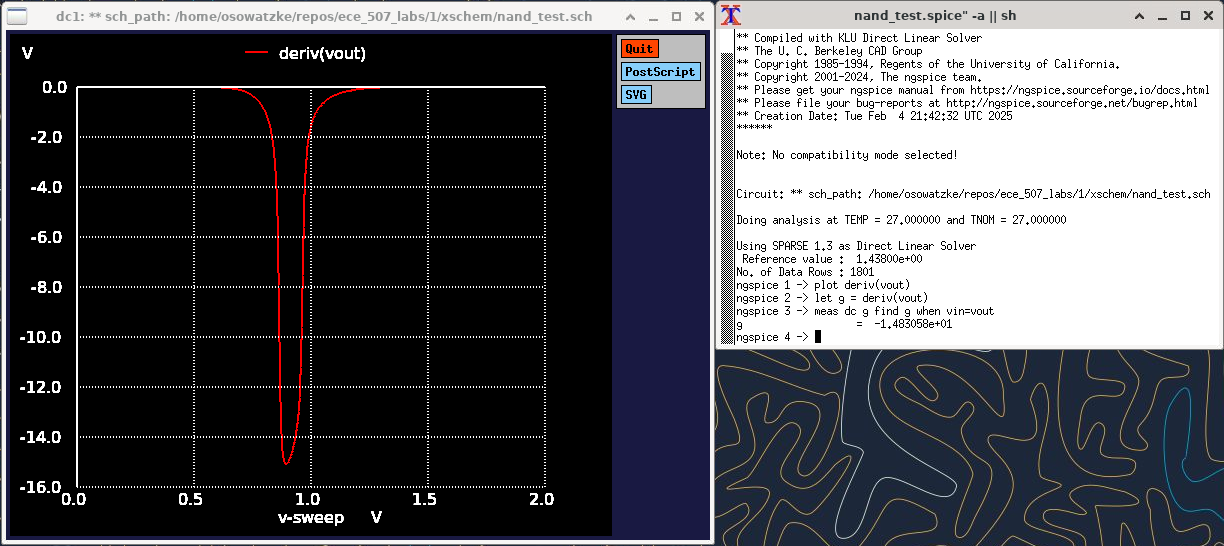
\includegraphics[width=0.8\textwidth]{nand_noise_analysis_g_sweep_va_vb.png}}
		\caption{NAND Gain Measurement}
		\label{fig::nand_noise_analysis_g_sweep_va_vb}
	\end{figure}
	
	\noindent With the updated values, we find that $V_{IL} \approx 0.8508\ \text{V}$ and $V_{IH} \approx 0.9722\ \text{V}$, which implies that $NM_L \approx 0.8508\ \text{V}$ and $NM_H \approx 0.8278\ \text{V}$. Compared to the values computed with the first-order MOSFET equations, these values are a significantly closer to our measured data.
	
	\subsection{Delay Analysis}
	
	In this section, we analyze the propagation delay of the NAND gate. To do so, we need to measure both the high-to-low propagation delay (\texttt{tphl}) and the low-to-high propagation delay (\texttt{tplh}). We measure \texttt{tphl} for each of the transitions listed in Table \ref{table::nand_gate_high_to_low_transitions}, and we measure \texttt{tplh} for each of the transitions listed in Table \ref{table::nand_gate_low_to_high_transitions}.
	
	\begin{table}[H]
	\begin{center}
	\caption{Inputs that Create Low-to-High Transition for NAND Gate}
	\label{table::nand_gate_low_to_high_transitions}
	\begin{tabular}{| c | c |}
		\hline
		\texttt{a} & \texttt{b} \\
		\hline	
		$1 \rightarrow 0$ & $1$\\
		\hline	
		$1$ & $1 \rightarrow 0$\\
		\hline	
		$1 \rightarrow 0$ & $1 \rightarrow 0$\\
		\hline
	\end{tabular}
	\end{center}
	\end{table}
	
	\noindent For variations of \texttt{a} with \texttt{b=1}, we can use the test circuit shown in Figure \ref{fig::nand_delay_test_sweep_va} to measure propagation delays. Note the input waveforms contains both rising an falling edges, so we can use it to measure \texttt{tphl} and \texttt{tplh}.

	\begin{figure}[H]
		\centerline{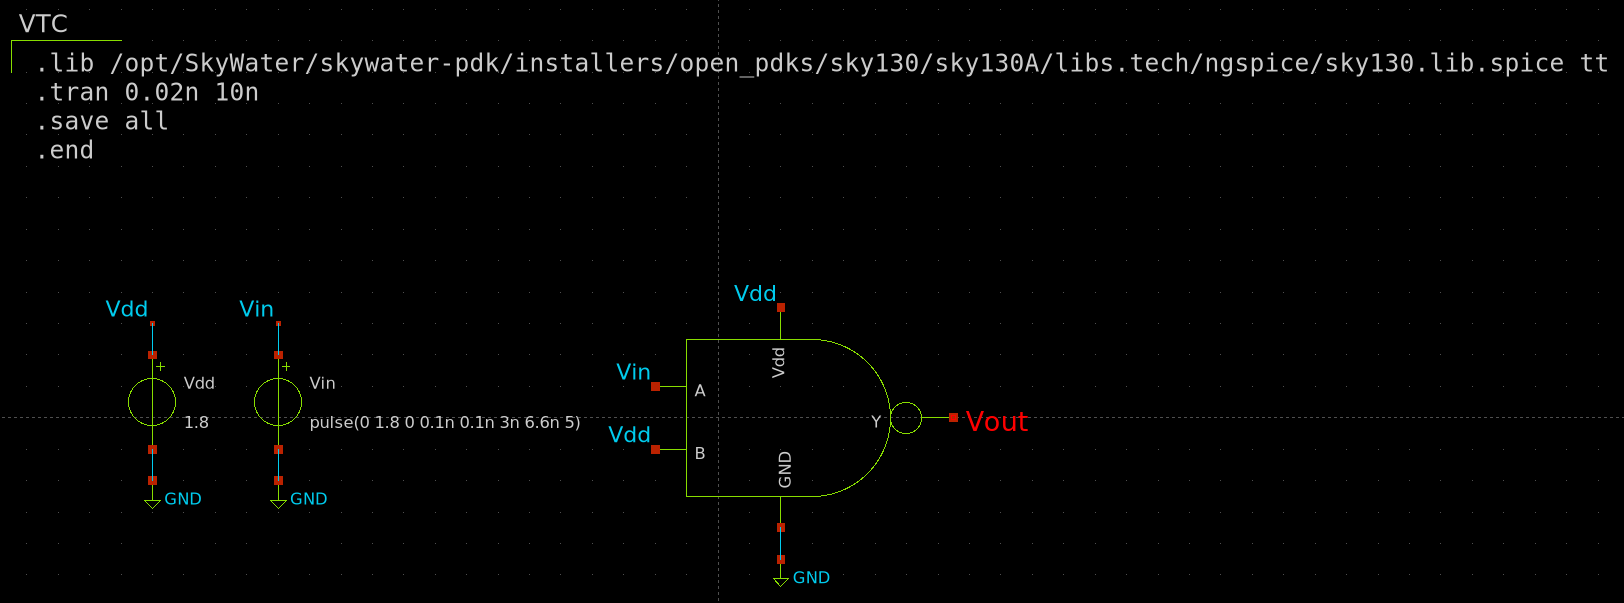
\includegraphics[width=0.8\textwidth]{nand_delay_test_sweep_va.png}}
		\caption{Test Circuit to Measure the Delay of the NAND Gate when \texttt{a} is Varied and \texttt{b=1}}
		\label{fig::nand_delay_test_sweep_va}
	\end{figure}
	
	\noindent Using the test circuit, we measure can measure \texttt{tphl} and \texttt{tplh} as follows:
	
	\begin{figure}[H]
		\centerline{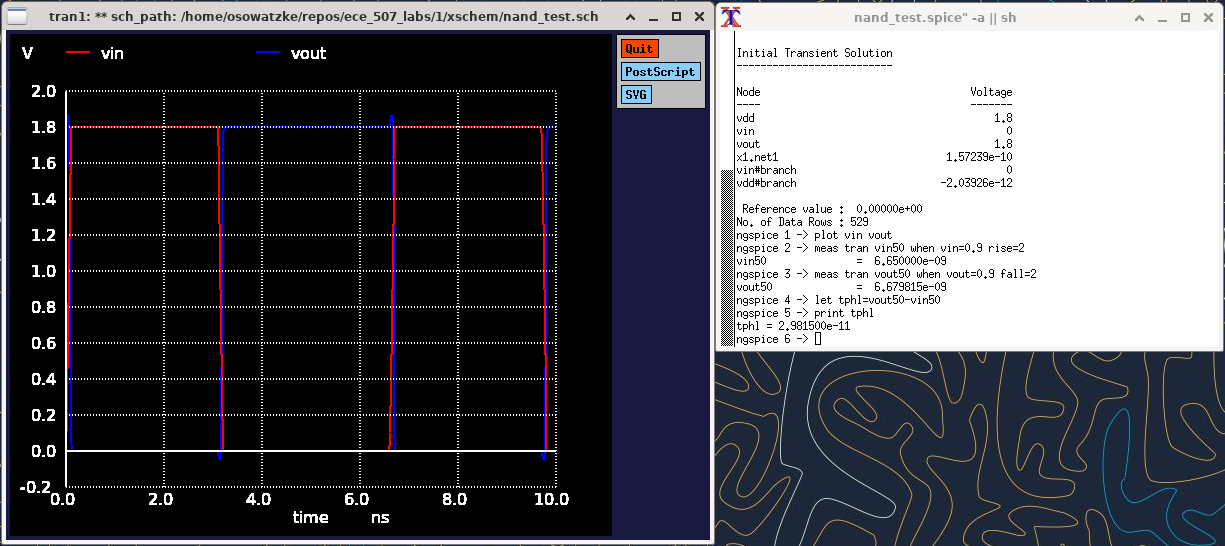
\includegraphics[width=0.8\textwidth]{nand_delay_sweep_va.png}}
		\caption{\texttt{tphl} Measurement for the NAND Gate when \texttt{a} is Varied and \texttt{b=1}}
		\label{fig::nand_delay_sweep_va}
	\end{figure}
	
	Examining the output results, we find that \texttt{tphl = 20.859 ps} for \texttt{a = }$0 \rightarrow 1$ and \texttt{b = 1}. Similarly, we find that \texttt{tphl = 33.178 ps} for \texttt{a = }$1 \rightarrow 0$ and \texttt{b = 1}. We perform similar analysis for the remaining transitions listed in Table \ref{table::nand_gate_high_to_low_transitions} and Table \ref{table::nand_gate_low_to_high_transitions}. Our results are summarized in Table \ref{table::nand_gate_delay_analysis}.
	
	\begin{table}[H]
	\begin{center}
	\caption{Propagation Delays for Each Transition That Result in an Output Logic Level Change}
	\label{table::nand_gate_delay_analysis}
	\begin{tabular}{| c | c | c || c | c | c |}
		\hline
		\texttt{a} & \texttt{b} & \texttt{tphl} & \texttt{a} & \texttt{b} & \texttt{tplh} \\
		\hline	
		$0 \rightarrow 1$ & $1$ & $20.859\ \text{ps}$ & $1 \rightarrow 0$ & $1$ & $33.178\ \text{ps}$\\
		\hline	
		$1$ & $0 \rightarrow 1$ & $28.146\ \text{ps}$ & $1$ & $1 \rightarrow 0$ & $48.137\ \text{ps}$\\
		\hline	
		$0 \rightarrow 1$ & $0 \rightarrow 1$ & $29.297\ \text{ps}$ & $1 \rightarrow 0$ & $1 \rightarrow 0$ & $26.097\ \text{ps}$\\
		\hline
	\end{tabular}
	\end{center}
	\end{table}
	
	We can compare our measurements to theoretical results. To get these results, we use the circuit shown in Figure \ref{fig::nand_eq_test_sweep_va_vb} to estimate the equivalent capacitance and resistance of the NAND gate when both inputs are swept together.
	
	\begin{figure}[H]
		\centerline{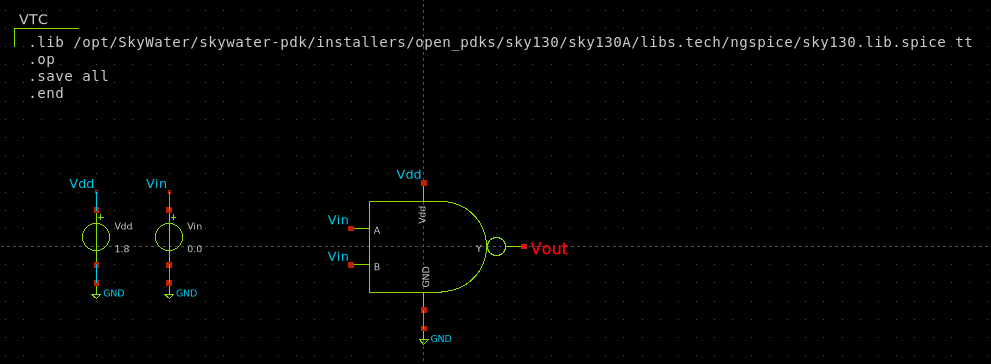
\includegraphics[width=0.8\textwidth]{nand_eq_test_sweep_va_vb.png}}
		\caption{Circuit to Estimate Equivalent Resistance and Capacitance of NAND Gate}
		\label{fig::nand_eq_test_sweep_va_vb}
	\end{figure}
	
	\noindent After running a simulation, we can extract the MOSFET names and their equivalent parameters as follows:
	
	\begin{figure}[H]
		\centerline{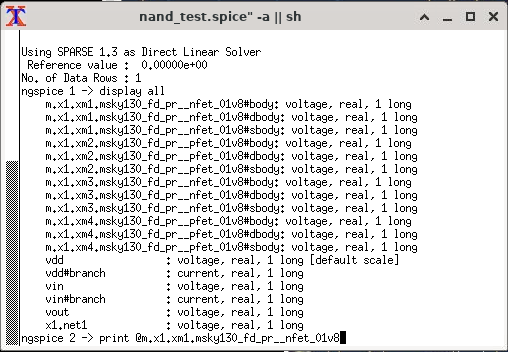
\includegraphics[width=0.4\textwidth]{nand_eq_display_sweep_va_vb.png}}
		\caption{Extracting MOSFET Names}
		\label{fig::nand_eq_display_sweep_va_vb}
	\end{figure}
	
	\begin{figure}[H]
		\centerline{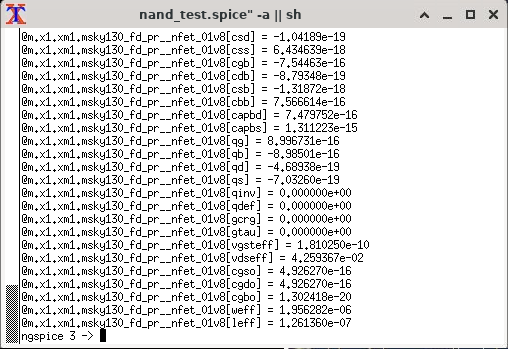
\includegraphics[width=0.4\textwidth]{nand_eq_params_sweep_va_vb.png}}
		\caption{M1 MOSFET Parameters}			\label{fig::nand_eq_params_sweep_va_vb}
	\end{figure}
	
	Using the provided methodology, we extract relevant parameters at $V_{DD}/2$. The values we measure at this input voltage are displayed in Table \ref{table::nand_gate_eq_params}.
	
	\begin{table}[H]
	\begin{center}
	\caption{Parameters Measured in SPICE Simulation}
	\label{table::nand_gate_eq_params}
	\begin{tabular}{| c | c | c |}
		\hline
		Transistor & $Cg$ & $R_{eq}$ \\
		\hline	
		\texttt{M1} & $1.444fF$ & $28.521k\Omega$ \\
		\hline
		\texttt{M2} & $1.868fF$ & $41.967k\Omega$ \\
		\hline
		\texttt{M3} & $1.761fF$ & $2.376k\Omega$ \\
		\hline
		\texttt{M4} & $1.868fF$ & $41.967k\Omega$ \\
		\hline
	\end{tabular}	
	\end{center}
	\end{table}
	
	\noindent The diffusion capacitances proved difficult to measure with this method. As a result, we estimated the diffusion capacitances with the gate capacitance, an approximation made by \cite{cmos_vlsi_design} for contacted diffusion. Additionally, because most our measurement windows were in the cutoff region, we approximated $C_{gs}$ and $C_{gd}$ as 0. 
	
	To find $t_{PLH}$, we consider the pull-up network. To find the propagation delay, we combine the parallel resistors and capacitors into a single parallel capacitor and resistor.
	
	\begin{equation}
		t_{PLH} = 0.69R_{eq}C_{eq} \approx 0.69(R_{M2}||R_{M4})(2C_{g_{M1}}) \approx 54.092\ \text{ps}
	\end{equation}
	
	\noindent To find $t_{PHL}$, we can solve for the Elmore delay of the pull-up network. Doing so we find:
	
	\begin{equation}
		t_{PHL} = 0.69R_{eq}C_{eq} \approx 0.69(2R_{M1}C_{g_{M1}} + 2(R_{M1} + R_{M3})C_{g_{M3}})\approx 131.920\ \text{ps}
	\end{equation}
	
	\noindent Our propagation delay estimates are off with respect to the measured data. This is likely occurring because of how we approximated the equivalent resistance. We found the equivalent resistance at a single point instead of integrating it over the measurement window. To get the equivalent resistance for $t_{PLH}$, our test circuit should have also forced $V_{in}$ to $0$ and measured the resistance while the output value was in range $[0, V_{DD}/2]$. Similarly, to get the equivalent resistance for $t_{PHL}$, our test circuit should have also forced $V_{in}$ to $V_{DD}$ and measured the resistance while the output value was in range $[V_{DD}, V_{DD}/2]$.
	
	\subsection{Power Analysis}
	
	In this section, we analyze the power consumption of our NAND gate. Similar to what we did above, we analyze the power consumption for each input variation that results in an output logical level change. For our input, we used a pulsed source. This allows us to capture both rising and falling edges of the output. We use the test circuit shown in Figure \ref{fig::nand_power_test_sweep_va} to measure the power consumption for variations of \texttt{a} with \texttt{b=1}. For this analysis, we have also attached a parasitic capacitance to the gate output.
	
	\begin{figure}[H]
		\centerline{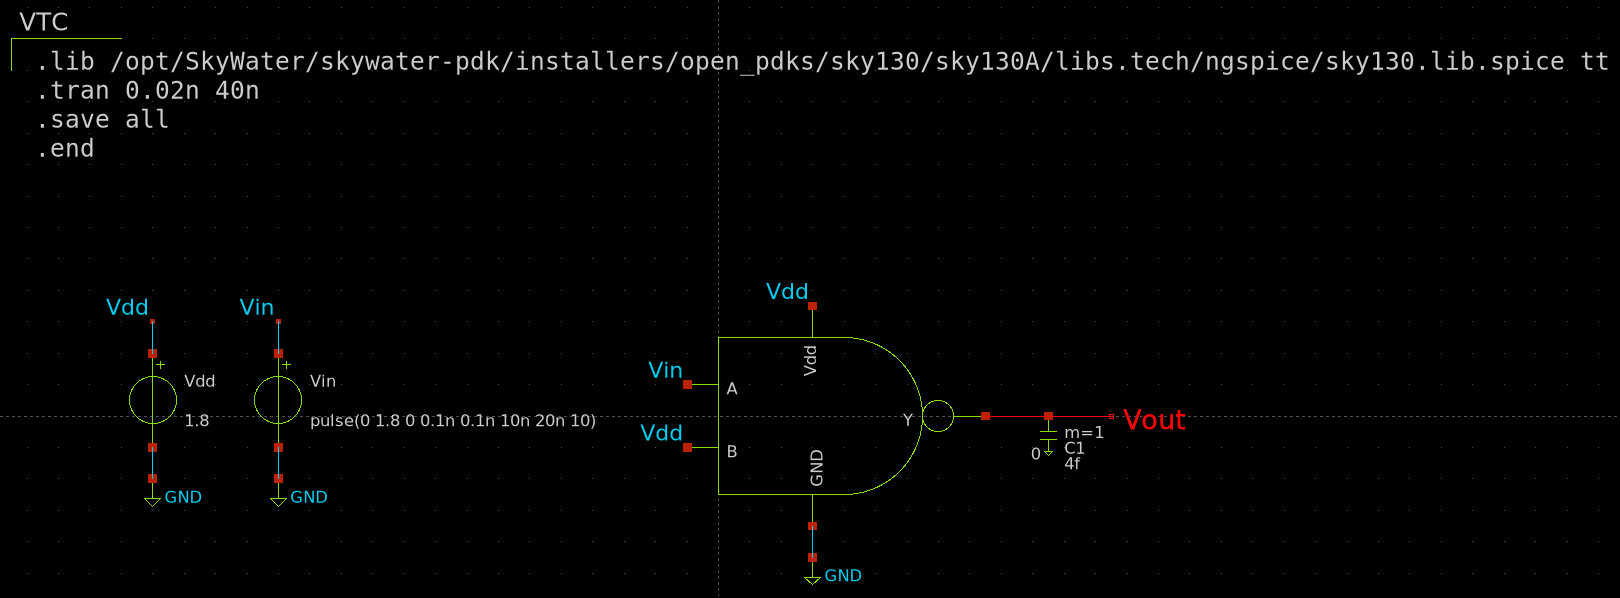
\includegraphics[width=0.8\textwidth]{nand_power_test_sweep_va.png}}
		\caption{Test Circuit to Measure the Power Consumption of the NAND Gate when \texttt{a} is Varied and \texttt{b=1}}
		\label{fig::nand_power_test_sweep_va}
	\end{figure}
	
	\noindent Using the test circuit, we measure the power consumption as follows:
	
	\begin{figure}[H]
		\centerline{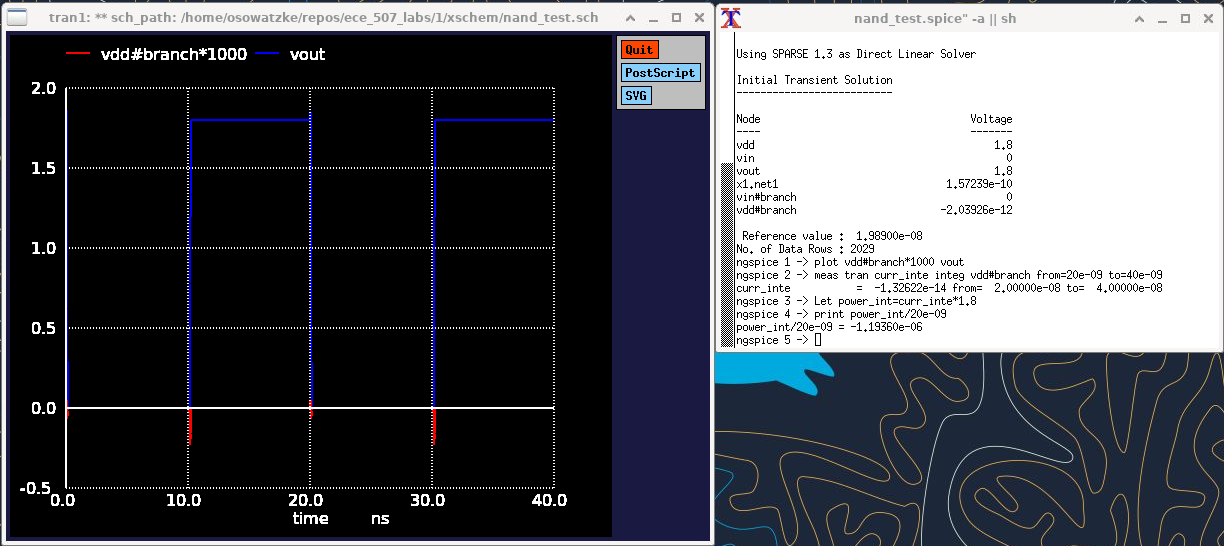
\includegraphics[width=0.8\textwidth]{nand_power_sweep_va.png}}
		\caption{Power Consumption of the NAND Gate when \texttt{a} is Varied and \texttt{b=1}}
		\label{fig::nand_power_sweep_va}
	\end{figure}
	
	\noindent Examining the results, we find that the power consumption is $1.34880{\mu}W$. Note that this power estimate includes the effects of the rising and falling edges of \texttt{a}. We can perform similar analysis for other variations of the input. Our results for this work are summarized in Table \ref{table::nand_gate_power_analysis}.
	
	\begin{table}[H]
	\begin{center}
	\caption{NAND Gate Power Consumption for Different Input Variations}
	\label{table::nand_gate_power_analysis}
	\begin{tabular}{| c | c | c |}
		\hline
		\texttt{a} & \texttt{b} & \texttt{Power}\\
		\hline	
		$0 \rightarrow 1 \rightarrow 0$ & $1$ & $1.34880{\mu}W$ \\
		\hline	
		$1$ & $0 \rightarrow 1 \rightarrow 0$ & $1.88943{\mu}W$ \\
		\hline	
		$0 \rightarrow 1 \rightarrow 0$ & $0 \rightarrow 1 \rightarrow 0$ & $1.44446{\mu}W$\\
		\hline
	\end{tabular}
	\end{center}
	\end{table}
	
	For comparison, we can also compute a theoretical power estimate for the case where both \texttt{a} and \texttt{b} switch together. The power consumption can be computed as follows:
	
	\begin{equation}
		P_{\text{total}} = P_{\text{dynamic}} + P_{\text{static}}
	\end{equation}
	
	\noindent where
	
	\begin{equation}
		P_{\text{dynamic}} = P_{\text{switching}} +  P_{\text{shortcircuit}}
	\end{equation}
	
	\noindent For a first-order estimate of the power, we ignore the static and short circuit power, which results in the following estimate:
	
	\begin{equation}
		P_{\text{total}} \approx P_{\text{switching}} = \alpha CV_{DD}^2f
	\end{equation}
	
	\noindent For our test setup, $\alpha = 1/2$ and $f = 1/(20 ns)$. For the capacitance, we need to consider the extrinsic intrinsic and instrinsic switching capacitances. The extrinsic capacitance is $4 fF$, and the intrinsic capacitance can be estimated by:
	
	 \begin{equation}
	 	\label{eq::nand_cint_est}
	 	C_int \approx 2C_{gp} + (C_{gn} + 2C_{gn})
	 \end{equation}
	 
	  \noindent where $C_{gp}$ and $C_{gn}$ are estimated using Table \ref{table::nand_gate_eq_params}. Letting $C_{gp} = 1.9 fF$ and $C_{gn} = 1.6 fF$, we find that $C_{int} \approx 8.6 fF$. Substituting, we find $P_{total} \approx 1.021 {\mu}W$. Note that this estimate is pretty close to the measured data. However, the fidelity of our estimate could be improved by considering the contribution of $P_{\text{static}}$ and $P_{\text{shortcircuit}}$.
	   
	\section{NOR Gate}
	
	In this section, we analyze the NOR gate built using SkyWater 130nm technology. We start by drawing a NOR gate and its corresponding symbol in xschem. Next, using ngspice, we analyze the voltage transfer characteristics of the gate, determining the switching threshold, $V_M$, and the noise margins. Then, using transient analysis, we measure the delay of the gate and its power consumption. For each value that we measure, we also compute a theoretical-equivalent using the equations provided in class.
	
	\subsection{Design}
	
	The NOR gate pull-down circuit is composed of two parallel NMOS transistors. The pull-up circuit is the complement of the pull-down circuit and is composed of two PMOS transistors in series. To determine the optimum sizing of the transistors in each network, we consider the equivalent resistance of each network. Compared to an inverter, the equivalent resistance of the pull-up network is doubled because the PMOS transistors are laid out in series. For the pull-down network, we consider the worst (slowest) case, in which only one NMOS transistor turns on. In this case, the pull-down network resistance is equivalent to that of an inverter. To account for differences in resistance, we need to double the width of the PMOS transistors, which halves their resistance. 
	
	For an inverter, we need to make the width of the PMOS transistor twice as large as the width of the NMOS transistor because the mobility of holes is lower than the mobility of electrons. After accounting for differences in resistances, we find that the PMOS width should be 4x larger than the NMOS width in a NOR gate. To match the behavior of the inverter with a NMOS width of 1 and a PMOS width of 2, we make the NMOS width 1 and the PMOS width 4. The NOR gate circuit with these transistor widths is shown in Figure \ref{fig::nor_schematic}.
	
	\begin{figure}[H]
		\centerline{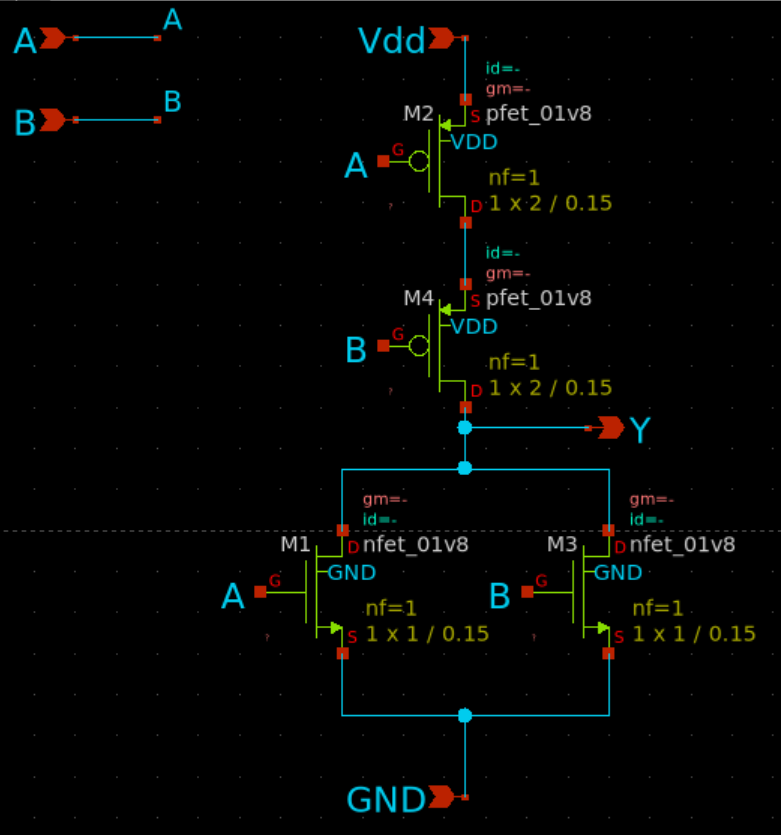
\includegraphics[width=0.4\textwidth]{nor_schematic.png}}
		\caption{NOR Circuit Schematic}
		\label{fig::nor_schematic}
	\end{figure}
	
	\noindent We also create a circuit symbol for the NOR gate, to allow reuse in other schematics. This circuit symbol is shown in Figure \ref{fig::nor_symbol}.
	
	\begin{figure}[H]
		\centerline{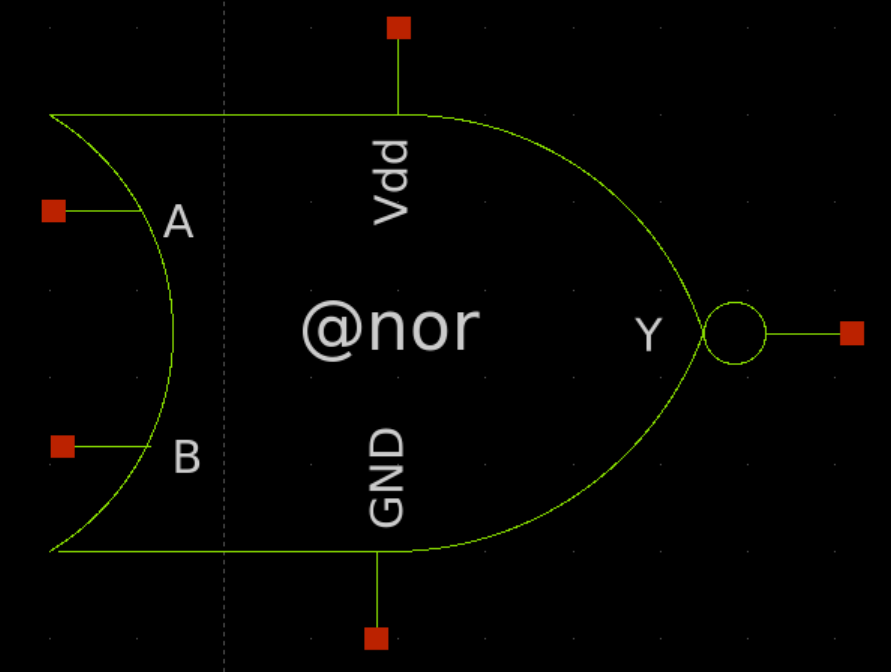
\includegraphics[width=0.4\textwidth]{nor_symbol.png}}
		\caption{NOR Circuit Symbol}
		\label{fig::nor_symbol}
	\end{figure}

	\subsection{Voltage Transfer Characteristics}
	
	In this section, we analyze the voltage transfer characteristics (VTC) of our NOR gate. For this analysis, we analyze the VTC for all combinations of inputs that lead to an output logic level change. When generating the VTC in ngspice, we consider consider only one set of transitions because the steady state output voltages are the same regardless of which direction we sweep. As such, we analyze the input voltages that result in high-to-low transitions. These voltages are dictated in Table \ref{table::nor_gate_high_to_low_transitions}.
	
	\begin{table}[H]
	\begin{center}
	\caption{Inputs that Create High to Low Transition for NOR Gate}
	\label{table::nor_gate_high_to_low_transitions}
	\begin{tabular}{| c | c |}
		\hline
		\texttt{a} & \texttt{b} \\
		\hline	
		$0 \rightarrow 1$ & $0$\\
		\hline	
		$0$ & $0 \rightarrow 1$\\
		\hline	
		$0 \rightarrow 1$ & $0 \rightarrow 1$\\
		\hline
	\end{tabular}
	\end{center}
	\end{table}
	
	The test circuit we use to generate the VTC for the first entry in the table is given in Figure \ref{fig::nor_vtc_test_sweep_va}.
	
	\begin{figure}[H]
		\centerline{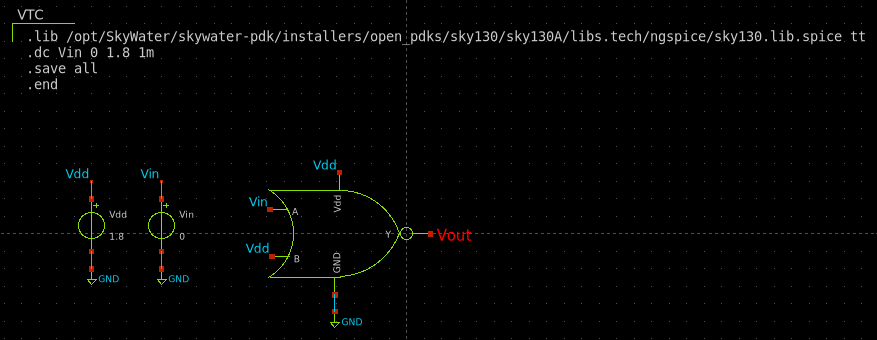
\includegraphics[width=0.8\textwidth]{nor_vtc_test_sweep_va.png}}
		\caption{NOR VTC Test Circuit for Variations of \texttt{a} with \texttt{b=0}}
		\label{fig::nor_vtc_test_sweep_va}
	\end{figure}	
	
	\noindent Using this test circuit, we perform DC analysis to generate the VTC and find $V_M$, which is the voltage at which $V_{in} = V_{out}$. The results of this analysis are shown in Figure \ref{fig::nor_vtc_sweep_va}.
	
	\begin{figure}[H]
		\centerline{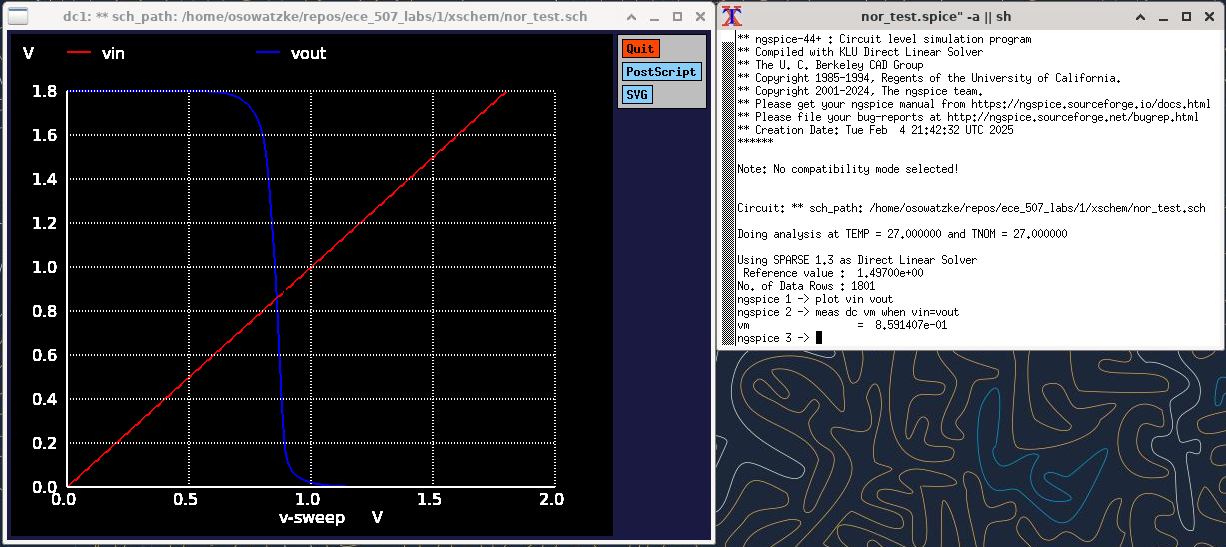
\includegraphics[width=0.8\textwidth]{nor_vtc_sweep_va.png}}
		\caption{NOR VTC Results for Variations of \texttt{a} with \texttt{b=0}}
		\label{fig::nor_vtc_sweep_va}
	\end{figure}
	
	Examining the results, we find that $V_M = 0.8952\ \text{V}$. With slight modifications to our test circuit, we can find $V_M$ for the other sets inputs listed in Table \ref{table::nor_gate_high_to_low_transitions}. These results are included in Table \ref{table::nor_gate_vm}.
	
	\begin{table}[H]
	\begin{center}
	\caption{\texttt{Vm} for Each Set of Inputs That Result in an Output Logic Level Change}
	\label{table::nor_gate_vm}
	\begin{tabular}{| c | c | c |}
		\hline
		\texttt{a} & \texttt{b} & \texttt{Vm}\\
		\hline	
		$0 \rightarrow 1$ & $0$ & $0.8952 \text{V}$\\
		\hline	
		$1$ & $0 \rightarrow 1$ & $0.8919 \text{V}$\\
		\hline	
		$0 \rightarrow 1$ & $0 \rightarrow 1$ & $0.8078 \text{V}$\\
		\hline
	\end{tabular}
	\end{center}
	\end{table}
	
	Reviewing our captured results, we see that $V_M$ is dependent on the gate inputs. $V_M$ is the smallest when both gates switch at the same time. This makes sense because our pull-down network is strongest in this case, causing $V_M$ to shift to the left.
	
	We can solve the IV equations to find $V_M$ analytically. However, that can get complicated, especially for gates more complex than an inverter. When both inputs switch at the same time, we can instead use an equivalent inverter model described in \cite{cmos_vlsi_design, equivalent_inverter, inverter_dc_analysis}. In the equivalent inverter model, we treat the gate as an inverter and scale the NMOS and PMOS transistors to reflect the series and parallel transistors. For parallel connections, the equivalent resistance will be halved, and for series connections, the equivalent resistance will be doubled. For an NOR gate, this is equivalent to doubling the NMOS width and halving PMOS width.
	
	\noindent We can use Equations \ref{eq::vm} and \ref{eq::beta_ratio} to solve for $V_M$ analytically. In Equation \ref{eq::beta_ratio}, we use the widths of the transistors in the equivalent inverter. Then, we can substitute parameters from Appendix \ref{appendix::nmos_iv_characteristics} and \ref{appendix::pmos_iv_characteristics}, to find $V_M$. Doing so, we find that $V_M \approx 0.8462\ \text{V}$. Note that this estimate is off for a few reasons. First, Equation \ref{eq::vm} assumes that both devices are operating in the velocity saturation state which is not the case here ($|V_{gs} - V_t| < |V_{DSAT}|$ for both the NMOS and PMOS transistors). Secondly, the first order model presented in class does not do a good job of modeling the current in the transition between linear and velocity saturation regions, where $V_M$ unfortunately defined.
	
	\subsection{Noise Analysis}
	
	Using the test circuit shown in Figure \ref{fig::nor_vtc_test_sweep_va}, we can also measure the noise margins, which are defined by Equations \ref{eq::noise_margin_high} and \ref{eq::noise_margin_low}. In the referenced formulas, $V_{IH}$ and $V_{IL}$ are defined as the unity points of the gain function, where the gain function is defined as the derivative of the VTC. For the case in which we vary \texttt{a} with \texttt{b=0}, we can identify the unity gain points and solve for the noise margins.
	
	\begin{figure}[H]
		\centerline{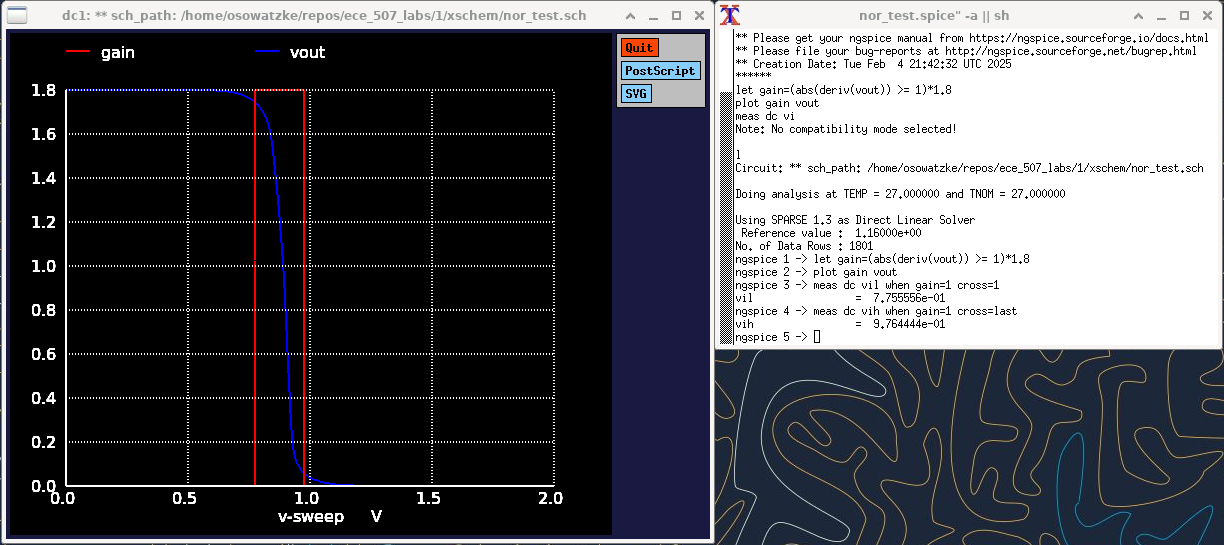
\includegraphics[width=0.8\textwidth]{nor_noise_analysis_sweep_va.png}}
		\caption{Measuring Noise Margins for the NOR Gate when \texttt{a} is Varied and \texttt{b=0}}	\label{fig::nor_noise_analysis_sweep_va}
	\end{figure}
	
	Examining the outputs shown in Figure \ref{fig::nor_noise_analysis_sweep_va}, we find that $V_{IL} = 0.7756\ \text{V}$ and $V_{IH} = 0.9764\ \text{V}$. This implies that $NM_{H} = 1.8\ \text{V} - 0.9764 \text{V} = 0.8326 \text{V}$ and $NM_{L} = 0.7756 \text{V} - 0 \text{V} = 0.7756 \text{V}$. With slight modifications to the test circuit, we can also measure the noise margins for the additional sets of inputs listed in Table \ref{table::nor_gate_high_to_low_transitions}. Our results for this analysis are listed in Table \ref{table::nor_gate_noise_analysis}.
	
	\begin{table}[H]
	\begin{center}
	\caption{Noise Margins for Each Set of Inputs That Result in an Output Logic Level Change}
	\label{table::nor_gate_noise_analysis}
	\begin{tabular}{| c | c | c | c | c | c |}
		\hline
		\texttt{a} & \texttt{b} & \texttt{Vih} & \texttt{Vil} & \texttt{Nmh} & \texttt{Nml} \\
		\hline	
		$0 \rightarrow 1$ & $0$ & $0.9764 \text{V}$ & $0.7756 \text{V}$ & $0.8326 \text{V}$ & $0.7756 \text{V}$\\
		\hline	
		$1$ & $0 \rightarrow 1$ & $1.0134 \text{V}$ & $0.7706 \text{V}$ & $0.7660 \text{V}$ & $0.7706 \text{V}$\\
		\hline	
		$0 \rightarrow 1$ & $0 \rightarrow 1$ & $0.7006 \text{V}$ & $0.8844 \text{V}$ & $0.9156 \text{V}$ & $0.7006 \text{V}$\\
		\hline
	\end{tabular}
	\end{center}
	\end{table}
	
	We can also compute the noise margins using the equations presented in class. For this analysis, we consider the case where \texttt{a} and \texttt{b} vary together. This allows us to analyze the circuit with an equivalent inverter model. To solve for the theoretical noise margins, we substitute values from Appendix \ref{appendix::nmos_iv_characteristics} and \ref{appendix::pmos_iv_characteristics} into equations \ref{eq::vih_theory} - \ref{eq::g_theory}. Doing so, we find that $g \approx -266$. If we then use our theoretical estimate of $V_{M}$, we find that $V_{IL} \approx 0.8426\ \text{V}$ and $V_{IH} \approx 0.8494\ \text{V}$, which implies that $NM_L = 0.8426\ \text{V}$ and $NM_H \approx 0.9506\ \text{V}$. Note that these values are significantly different than our measured values. As discussed above, this occurs for two reasons. First, $V_M$ is not in the velocity saturation region. Second, the level 1 model equations do not fit the transition between linear and velocity saturation regions well.
	
	To improve the quality of our theoretical noise margin estimates, we can also use parameters measured in ngspice. We specifically use $V_M = 0.8078 V$ and $g = -18.35$, where $g$ is computed in Figure \ref{fig::nor_noise_analysis_g_sweep_va_vb}.
	
	\begin{figure}[H]
		\centerline{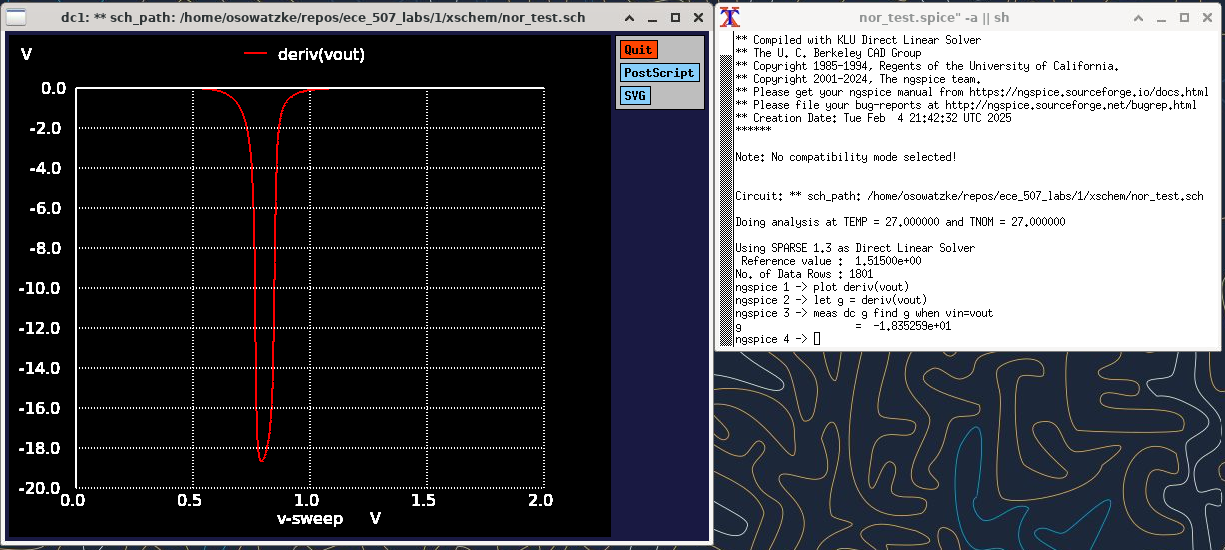
\includegraphics[width=0.8\textwidth]{nor_noise_analysis_g_sweep_va_vb.png}}
		\caption{NOR Gain Measurement}
		\label{fig::nor_noise_analysis_g_sweep_va_vb}
	\end{figure}
	
	\noindent With the updated values, we find that $V_{IL} \approx 0.7537\ \text{V}$ and $V_{IH} \approx 0.8518\ \text{V}$, which implies that $NM_L = 0.7537\ \text{V}$ and $NM_H \approx 0.9482\ \text{V}$. Compared to the values computed with the first-order MOSFET equations, these values are a significantly closer to our measured data.
	
	\subsection{Delay Analysis}
	
	In this section, we analyze the propagation delay of the NOR gate. To do so, we need to measure both the high-to-low propagation delay (\texttt{tphl}) and the low-to-high propagation delay (\texttt{tplh}). We measure \texttt{tphl} for each of the transitions listed in Table \ref{table::nor_gate_high_to_low_transitions}, and we measure \texttt{tplh} for each of the transitions listed in Table \ref{table::nor_gate_low_to_high_transitions}.
	
	\begin{table}[H]
	\begin{center}
	\caption{Inputs that Create Low-to-High Transition for NOR Gate}
	\label{table::nor_gate_low_to_high_transitions}
	\begin{tabular}{| c | c |}
		\hline
		\texttt{a} & \texttt{b} \\
		\hline	
		$1 \rightarrow 0$ & $0$\\
		\hline	
		$0$ & $1 \rightarrow 0$\\
		\hline	
		$1 \rightarrow 0$ & $1 \rightarrow 0$\\
		\hline
	\end{tabular}
	\end{center}
	\end{table}
	
	\noindent For variations of \texttt{a} with \texttt{b=0}, we can use the test circuit shown in Figure \ref{fig::nor_delay_test_sweep_va} to measure propagation delays. Note the input waveforms contains both rising an falling edges, so we can use it to measure \texttt{tphl} and \texttt{tplh}.

	\begin{figure}[H]
		\centerline{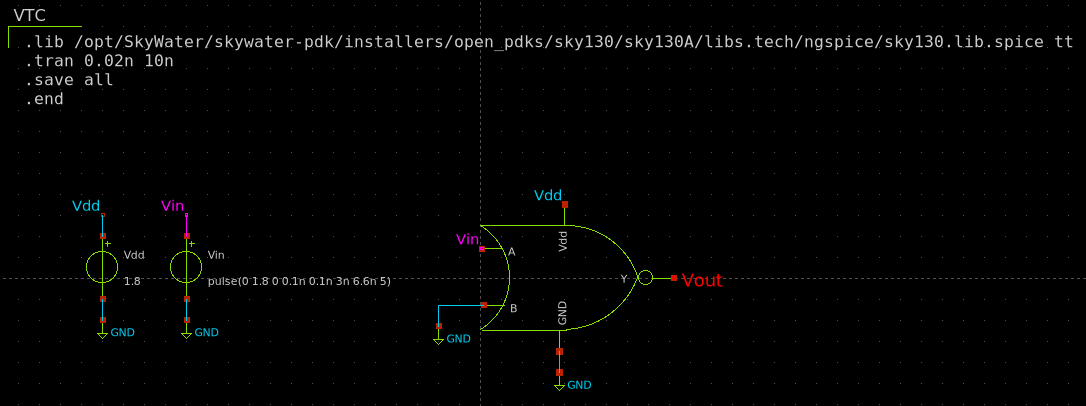
\includegraphics[width=0.8\textwidth]{nor_delay_test_sweep_va.png}}
		\caption{Test Circuit to Measure the Delay of the NOR Gate when \texttt{a} is Varied and \texttt{b=0}}
		\label{fig::nor_delay_test_sweep_va}
	\end{figure}
	
	\noindent Using the test circuit, we measure can measure \texttt{tphl} and \texttt{tplh} as follows:
	
	\begin{figure}[H]
		\centerline{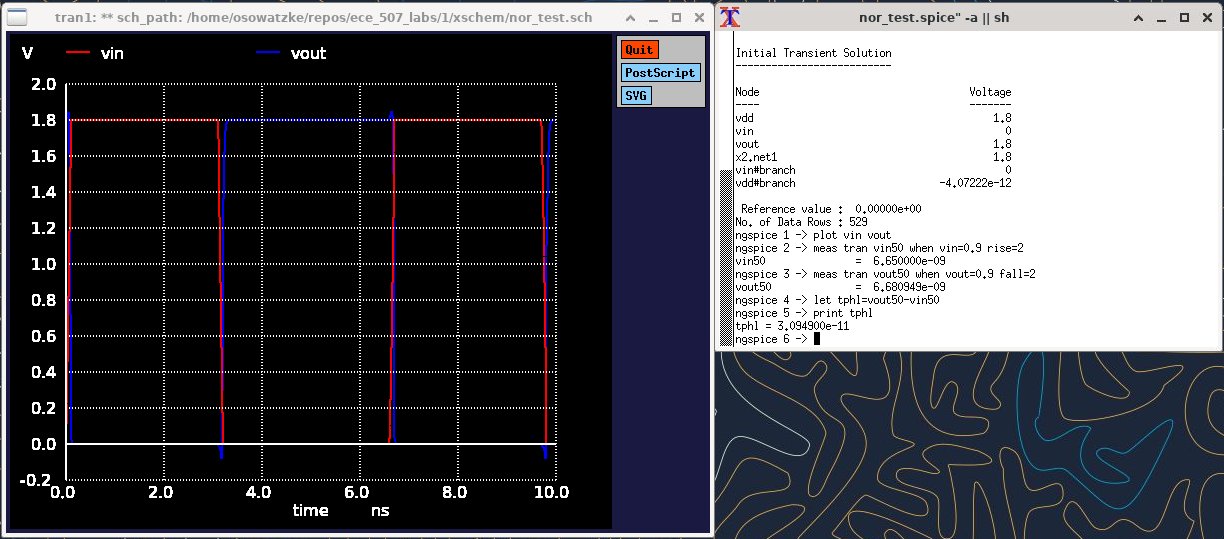
\includegraphics[width=0.8\textwidth]{nor_delay_sweep_va.png}}
		\caption{\texttt{tphl} Measurement for the NAND Gate when \texttt{a} is Varied and \texttt{b=0}}
		\label{fig::nor_delay_sweep_va}
	\end{figure}
	
	Examining the output results, we find that \texttt{tphl = 44.975 ps} for \texttt{a = }$0 \rightarrow 1$ and \texttt{b = 1}. Similarly, we find that \texttt{tphl = 45.841 ps} for \texttt{a = }$1 \rightarrow 0$ and \texttt{b = 0}. We perform similar analysis for the remaining transitions listed in Table \ref{table::nor_gate_high_to_low_transitions} and Table \ref{table::nor_gate_low_to_high_transitions}. Our results are summarized in Table \ref{table::nor_gate_delay_analysis}.
	
	\begin{table}[H]
	\begin{center}
	\caption{Propagation Delays for Each Transition That Result in an Output Logic Level Change}
	\label{table::nor_gate_delay_analysis}
	\begin{tabular}{| c | c | c || c | c | c |}
		\hline
		\texttt{a} & \texttt{b} & \texttt{tphl} & \texttt{a} & \texttt{b} & \texttt{tplh} \\
		\hline	
		$0 \rightarrow 1$ & $0$ & $44.975\ \text{ps}$ & $1 \rightarrow 0$ & $0$ & $45.841\ \text{ps}$\\
		\hline	
		$0$ & $0 \rightarrow 1$ & $29.139\ \text{ps}$ & $0$ & $1 \rightarrow 0$ & $29.942\ \text{ps}$\\
		\hline	
		$0 \rightarrow 1$ & $0 \rightarrow 1$ & $22.437\ \text{ps}$ & $1 \rightarrow 0$ & $1 \rightarrow 0$ & $40.997\ \text{ps}$\\
		\hline
	\end{tabular}
	\end{center}
	\end{table}
	
	We can compare our measurements to theoretical results. To get these results, we use the circuit shown in Figure \ref{fig::nor_eq_test_sweep_va_vb} to estimate the equivalent capacitance and resistance of the NOR gate when both inputs are swept together.
	
	\begin{figure}[H]
		\centerline{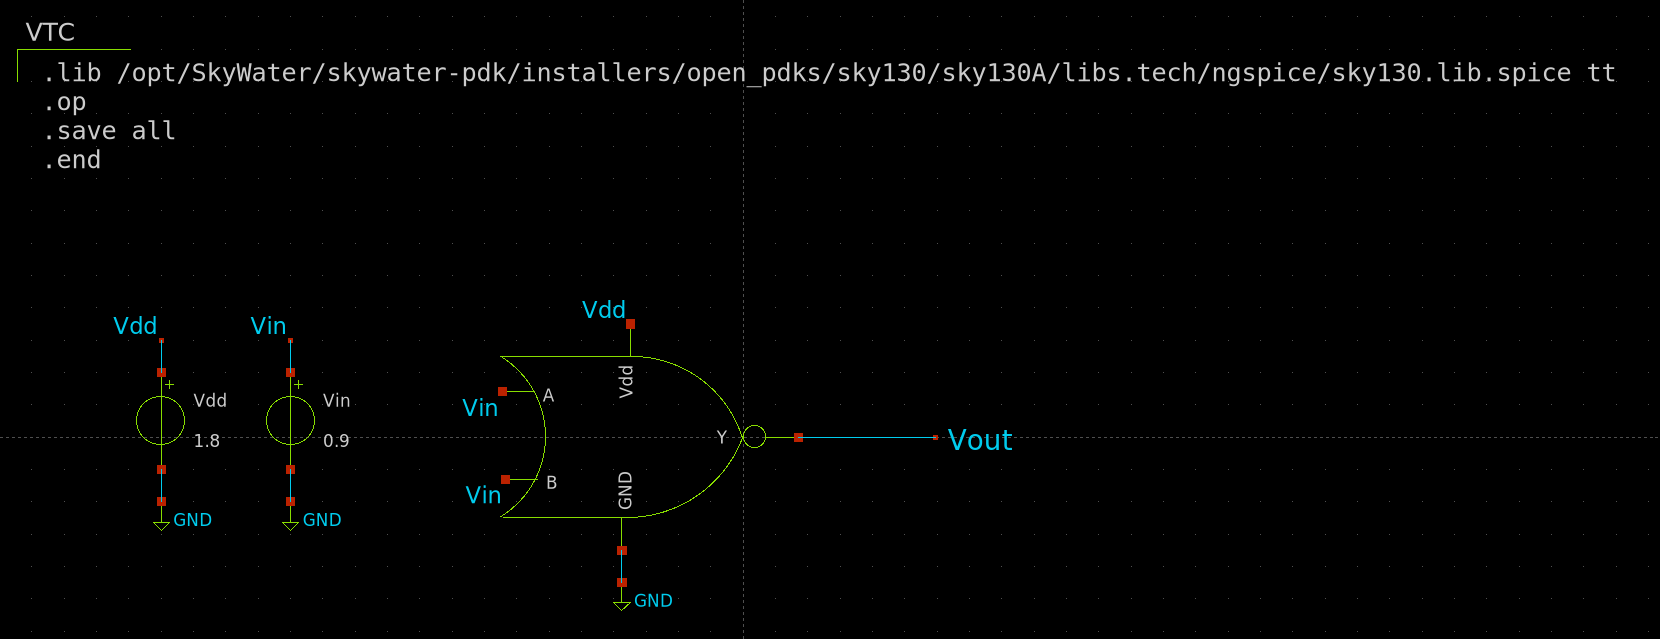
\includegraphics[width=0.8\textwidth]{nor_eq_test_sweep_va_vb.png}}
		\caption{Circuit to Estimate Equivalent Resistance and Capacitance of NOR Gate}
		\label{fig::nor_eq_test_sweep_va_vb}
	\end{figure}
	
	\noindent After running a simulation, we can extract the MOSFET names and their equivalent parameters as follows:
	
	\begin{figure}[H]
		\centerline{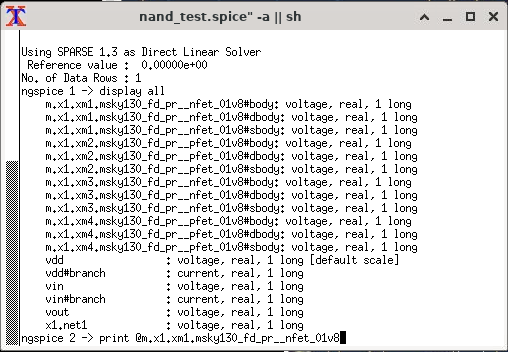
\includegraphics[width=0.4\textwidth]{nand_eq_display_sweep_va_vb.png}}
		\caption{Extracting MOSFET Names}
		\label{fig::nor_eq_display_sweep_va_vb}
	\end{figure}
	
	\begin{figure}[H]
		\centerline{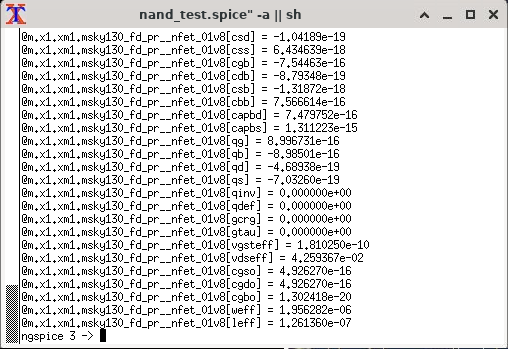
\includegraphics[width=0.4\textwidth]{nand_eq_params_sweep_va_vb.png}}
		\caption{M1 MOSFET Parameters}			\label{fig::nor_eq_params_sweep_va_vb}
	\end{figure}
	
	Using the provided methodology, we extract relevant parameters at $V_{DD}/2$. The values we measure at this input voltage are displayed in Table \ref{table::nor_gate_eq_params}.
	
	\begin{table}[H]
	\begin{center}
	\caption{Parameters Measured in SPICE Simulation}
	\label{table::nor_gate_eq_params}
	\begin{tabular}{| c | c | c |}
		\hline
		Transistor & $Cg$ & $R_{eq}$ \\
		\hline	
		\texttt{M1} & $0.899fF$ & $4.652k\Omega$ \\
		\hline
		\texttt{M2} & $3.709fF$ & $10.651k\Omega$ \\
		\hline
		\texttt{M3} & $0.899fF$ & $4.652k\Omega$ \\
		\hline
		\texttt{M4} & $3.543fF$ & $110.998k\Omega$ \\
		\hline
	\end{tabular}	
	\end{center}
	\end{table}
	
	\noindent The diffusion capacitances proved difficult to measure with this method. As a result, we estimated the diffusion capacitances with the gate capacitance, an approximation made by \cite{cmos_vlsi_design} for contacted diffusion. Additionally, because most our measurement windows were in the cutoff region, we approximated $C_{gs}$ and $C_{gd}$ as 0. 
	
	To find $t_{PHL}$, we consider the pull-down network. To find the propagation delay, we combine the parallel resistors and capacitors into a single parallel capacitor and resistor.
	
	\begin{equation}
		t_{PLH} = 0.69R_{eq}C_{eq} \approx 0.69(R_{M1}||R_{M3})(2C_{g_{M1}}) \approx 5.771\ \text{ps}
	\end{equation}
	
	\noindent To find $t_{PHL}$, we can solve for the Elmore delay of the pull-up network. Doing so we find:
	
	\begin{equation}
		t_{PHL} = 0.69R_{eq}C_{eq} \approx 0.69(2R_{M2}C_{g_{M2}} + 2(R_{M2} + R_{M4})C_{g_{M4}})\approx 594.783\ \text{ps}
	\end{equation}
	
	Our propagation delay estimates are off with respect to the measured data. This is likely occurring because of how we approximated the equivalent resistance. We found the equivalent resistance at a single point instead of integrating it over the measurement window. To get the equivalent resistance for $t_{PLH}$, our test circuit should have also forced $V_{in}$ to $0$ and measured the resistance while the output value was in range $[0, V_{DD}/2]$. Similarly, to get the equivalent resistance for $t_{PHL}$, our test circuit should have also forced $V_{in}$ to $V_{DD}$ and measured the resistance while the output value was in range $[V_{DD}, V_{DD}/2]$.
	
	\subsection{Power Analysis}
	
	In this section, we analyze the power consumption of our NOR gate. Similar to what we did above, we analyze the power consumption for each input variation that results in an output logical level change. For our input, we used a pulsed source. This allows us to capture both rising and falling edges of the output. We use the test circuit shown in Figure \ref{fig::nor_power_test_sweep_va} to measure the power consumption for variations of \texttt{a} with \texttt{b=0}. For this analysis, we have also attached a parasitic capacitance to the gate output.
	
	\begin{figure}[H]
		\centerline{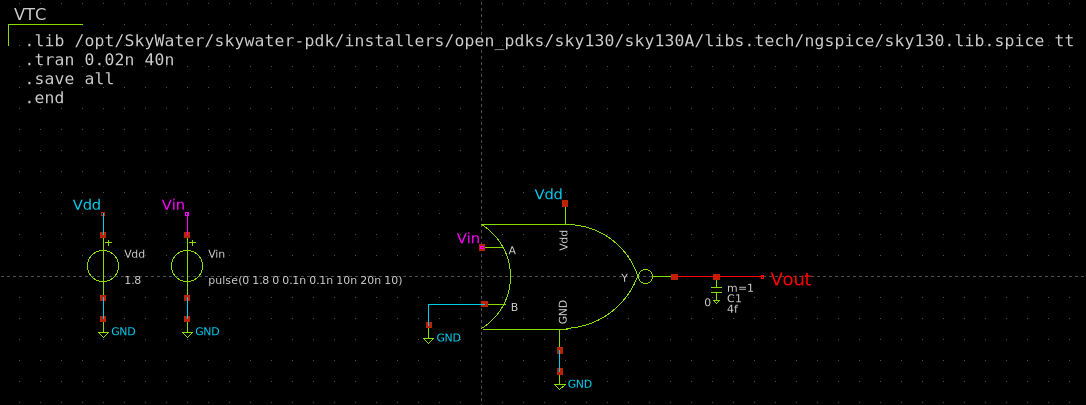
\includegraphics[width=0.8\textwidth]{nor_power_test_sweep_va.png}}
		\caption{Test Circuit to Measure the Power Consumption of the NOR Gate when \texttt{a} is Varied and \texttt{b=0}}
		\label{fig::nor_power_test_sweep_va}
	\end{figure}
	
	\noindent Using the test circuit, we measure the power consumption as follows:
	
	\begin{figure}[H]
		\centerline{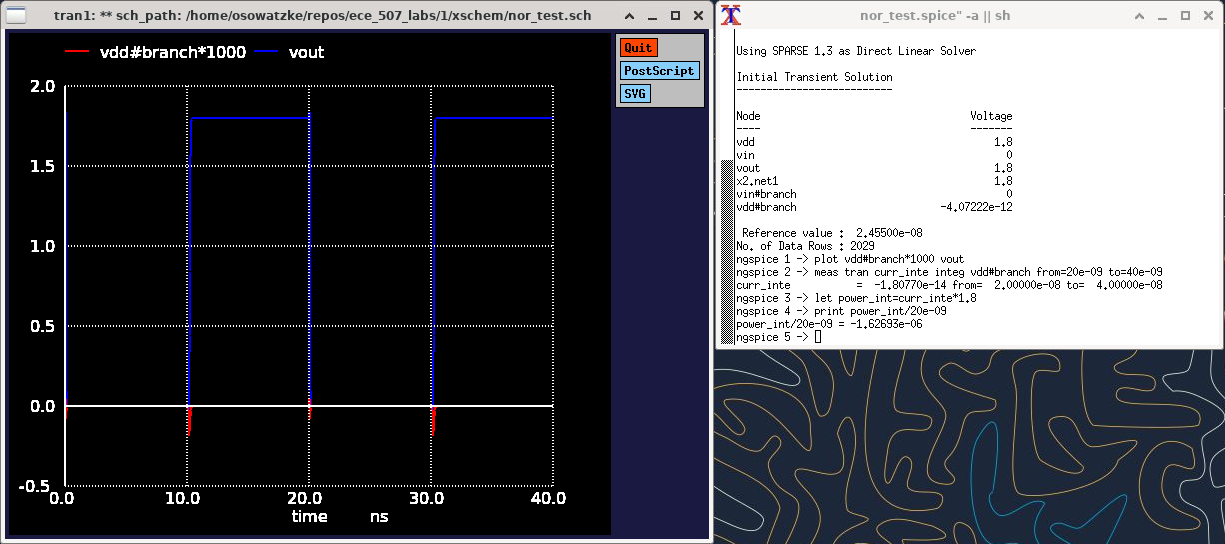
\includegraphics[width=0.8\textwidth]{nor_power_sweep_va.png}}
		\caption{Power Consumption of the NOR Gate when \texttt{a} is Varied and \texttt{b=0}}
		\label{fig::nor_power_sweep_va}
	\end{figure}
	
	\noindent Examining the results, we find that the power consumption is $2.28022{\mu}W$. Note that this power estimate includes the effects of the rising and falling edges of \texttt{a}. We can perform similar analysis for other variations of the input. Our results for this work are summarized in Table \ref{table::nor_gate_power_analysis}.
	
	\begin{table}[H]
	\begin{center}
	\caption{NOR Gate Power Consumption for Different Input Variations}
	\label{table::nor_gate_power_analysis}
	\begin{tabular}{| c | c | c |}
		\hline
		\texttt{a} & \texttt{b} & \texttt{Power}\\
		\hline	
		$0 \rightarrow 1 \rightarrow 0$ & $1$ & $2.28022{\mu}W$ \\
		\hline	
		$1$ & $0 \rightarrow 1 \rightarrow 0$ & $1.3767{\mu}W$ \\
		\hline	
		$0 \rightarrow 1 \rightarrow 0$ & $0 \rightarrow 1 \rightarrow 0$ & $1.61932{\mu}W$\\
		\hline
	\end{tabular}
	\end{center}
	\end{table}
	
	For comparison, we can also compute a theoretical power estimate for the case where both \texttt{a} and \texttt{b} switch together. The power consumption can be computed as follows:
	
	\begin{equation}
		P_{\text{total}} = P_{\text{dynamic}} + P_{\text{static}}
	\end{equation}
	
	\noindent where
	
	\begin{equation}
		P_{\text{dynamic}} = P_{\text{switching}} +  P_{\text{shortcircuit}}
	\end{equation}
	
	\noindent For a first-order estimate of the power, we ignore the static and short circuit power, which results in the following estimate:
	
	\begin{equation}
		P_{\text{total}} \approx P_{\text{switching}} = \alpha CV_{DD}^2f
	\end{equation}
	
	\noindent For our test setup, $\alpha = 1/2$ and $f = 1/(20 ns)$. For the capacitance, we need to consider the extrinsic intrinsic and instrinsic switching capacitances. The extrinsic capacitance is $4 fF$, and the intrinsic capacitance can be estimated by:
	
	 \begin{equation}
	 	\label{eq::cint_est}
	 	C_int \approx (2C_{gp} + C_{gp}) + 2C_{gn}
	 \end{equation}
	 
	  \noindent where $C_{gp}$ and $C_{gn}$ are estimated using Table \ref{table::nor_gate_eq_params}. Letting $C_{gp} = 3.6 fF$ and $C_{gn} = 0.9 fF$, we find that $C_{int} \approx 12.6 fF$. Substituting, we find $P_{total} \approx 1.345 {\mu}W$. Note that this estimate is pretty close to the measured data. However, the fidelity of our estimate could be improved by considering the contribution of $P_{\text{static}}$ and $P_{\text{shortcircuit}}$.
	
	\subsection{Conclusion}
	
	In this lab, we used xschem to draw and simulate NAND and NOR gates built using SkyWater 130nm technology. To balance the equivalent resistance of the pull-up and pull-down networks, we learned that we had to modify the widths of the transistors in each network. In the NAND gate, we specifically doubled the widths of the NMOS gates, while keeping the widths of the PMOS gates constant. Similarly, for the NOR gate, we doubled the widths of the PMOS gates, while keeping the widths of the NMOS gates constant. Following the procedure described for the inverter, we also determined the voltage transfer characteristics, noise margins, delay, and power of each gate. For comparison, we also used the equations presented in class to theoretically compute these parameters. The equations presented in class proved difficult to analyze for each of the gates. As a result, we used the equivalent inverter model to simplify our analysis. However, our theoretical analysis proved to be a poor fit for the measured data for a couple reasons. First, the equations presented in class assumed that the transistors were in the velocity saturation, which was not the case in most of our equations. Additionally, the level 1 mosfet models we used for our theoretical analysis proved to be a poor fit for the IV data in between the resistive and velocity saturation regions.
	
	\bibliographystyle{IEEEtran}
	\bibliography{IEEEabrv,sources}
	\pagebreak
	\appendix
	\section{NMOS IV Characteristics}
	\label{appendix::nmos_iv_characteristics}
	
	In this appendix, we fit a first-order mosfet model to NMOS IV characteristics measured with the sky130A PDK. This enables us to use the equations presented in class to perform first-order analysis of our CMOS gate. We start by estimating the threshold voltage of the NMOS transistor. To perform this measurement, we use the linear extrapolation (or maximum gm) method given in \cite{cmos_vlsi_design}. Our ngspice flowchart for this analysis is given in Figure \ref{fig::nmos_vt_meas_schem}.
	
	\begin{figure}[H]
		\centerline{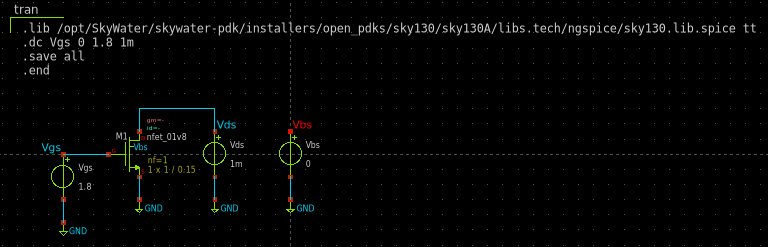
\includegraphics[width=0.8\textwidth]{nmos_vt_meas_schem.png}}
		\caption{NGSPICE Schematic Used to Measure the NMOS Threshold Voltage}
		\label{fig::nmos_vt_meas_schem}
	\end{figure}
	
	\noindent Using the flowchart, we examine the drain current for the NMOS transistor in the linear region of operation. In this region, the drain current of the NMOS transistor is given as follows:
	
	\begin{equation}
		I_{ds} = k_n\frac{W_n}{L}\left(V_{gs} - V_{t_n} - \frac{V_{ds}}{2}\right)V_{ds}
	\end{equation}
	
	\noindent To fit the IV characteristics, we estimate the $I_{ds}$ curve with a line that is tangent to the point with maximum-slope. We then define $V_t$ as the voltage at which the estimated current is zero. This procedure is illustrated in Figure \ref{fig::nmos_vt_meas}, which predicts a threshold voltage of 0.759 V.
	
	\begin{figure}[H]
		\centerline{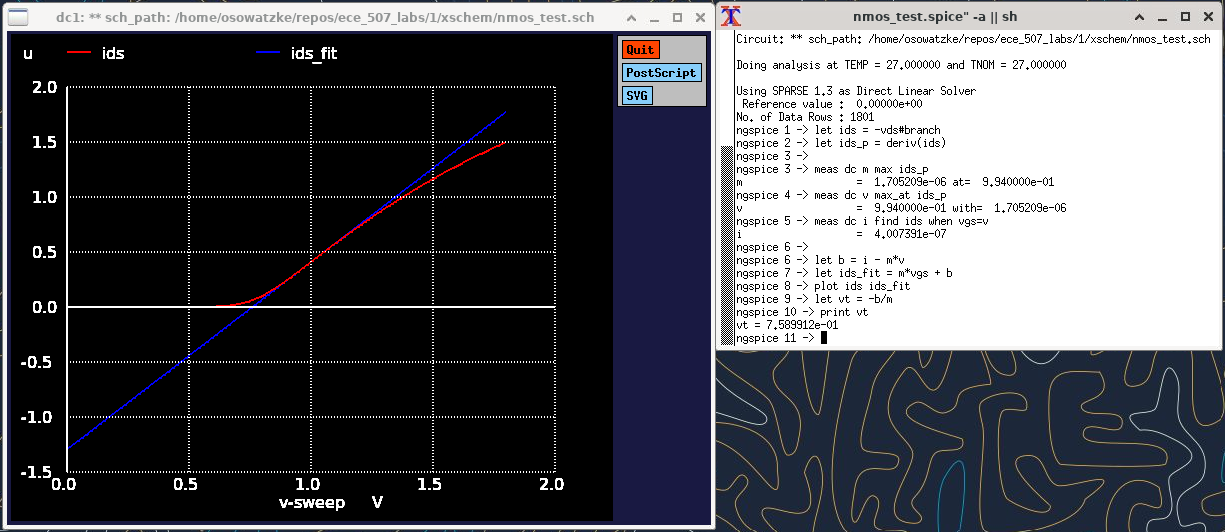
\includegraphics[width=0.8\textwidth]{nmos_vt_meas.png}}
		\caption{Estimating NMOS Threshold Voltage}
		\label{fig::nmos_vt_meas}
	\end{figure}
	
	Next, we measure the saturation voltage. We use the flowchart shown in Figure \ref{fig::nmos_vt_meas_schem} to perform this measurement.
	
	\begin{figure}[H]
		\centerline{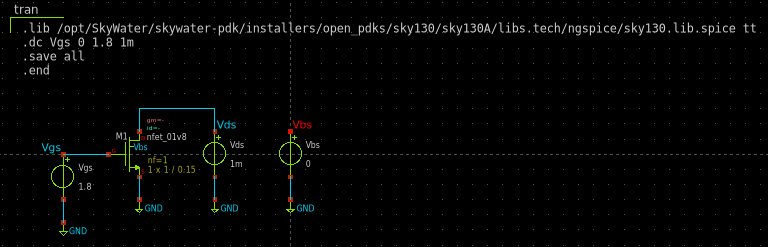
\includegraphics[width=0.8\textwidth]{nmos_vt_meas_schem.png}}
		\caption{NGSPICE Schematic Used to Measure the NMOS Saturation Voltage}
		\label{fig::nmos_vdsat_meas_schem}
	\end{figure}
	
	 \noindent In the above schematic, we consider the drain current in the velocity saturation region. The drain current in this region is defined as follows:
	
	\begin{equation}
		\label{eq::nmos_sat_current}
		I_{ds} = k_n\frac{W_n}{L}\left(V_{gs} - V_{t_n} - \frac{V_{DSAT_n}}{2}\right)V_{DSAT_n}(1 + {\lambda}V_{ds})
	\end{equation}
	
	\noindent If we analyze the ratio of drain currents for the same values of $V_{ds}$ and different values of $V_{gs}$, we can express the ratios as follows:
	
	\begin{equation}
		\frac{V_{gs_1} - V_{t_n} - V_{DSAT_n}/2}{V_{gs_2} - V_{t_n} - V_{DSAT_n}/2} = \frac{V_{gs_1} - V}{V_{gs_2} - V} = \frac{I_{ds_1}}{I_{ds_2}} = \alpha
	\end{equation}
	
	\noindent Solving for $V$, we obtain the following:
	
	\begin{equation}
		V = \frac{{\alpha}V_{gs_2} - V_{gs_1}}{\alpha - 1}
	\end{equation}
	
	\noindent where $V_{DSAT_n} = 2(V - V_{t_n})$. Following the procedure outlined above, we execute the following commands in ngspice to derive the saturation voltage. Our work is shown in Figure \ref{fig::nmos_vt_meas_schem} and we find that $V_{DSAT_n} = 0.202\ \text{V}$.
	
	\begin{figure}[H]
		\centerline{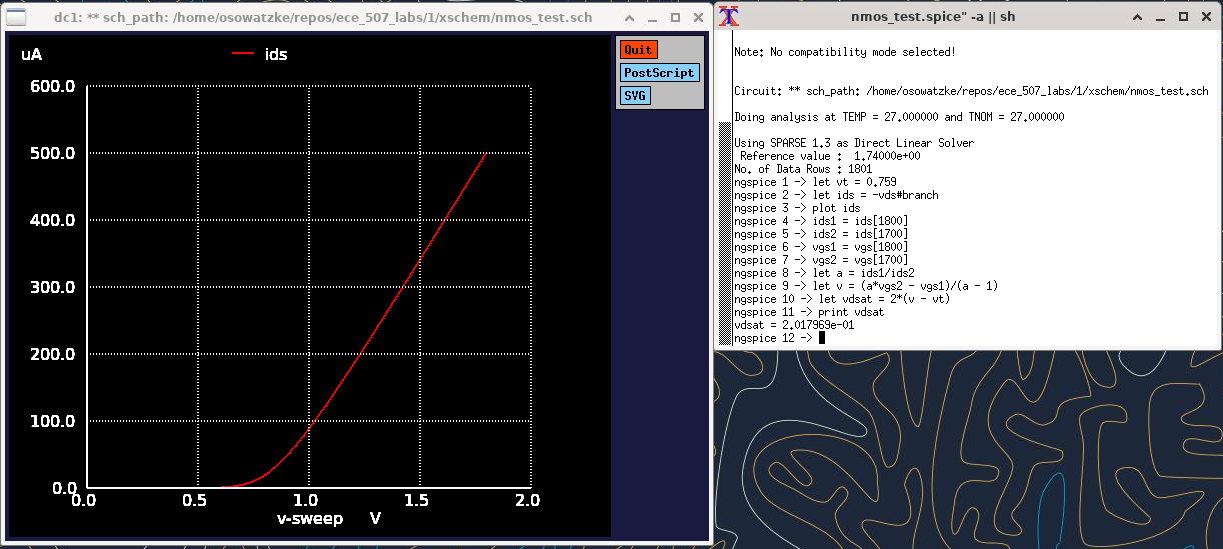
\includegraphics[width=0.8\textwidth]{nmos_vdsat_meas.png}}
		\caption{Measuring the NMOS Saturation Voltage}
		\label{fig::nmos_vdsat_meas}
	\end{figure}
	
	Then, we find the channel length modulation coefficient $\lambda$. To do this, we use the NGSPICE schematic shown in Figure \ref{fig::nmos_lambda_meas_schem}.
	
	\begin{figure}[H]
		\centerline{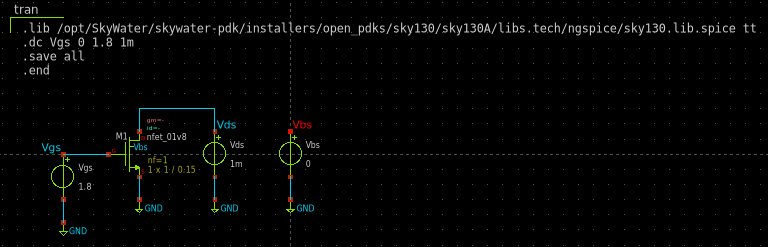
\includegraphics[width=0.8\textwidth]{nmos_vt_meas_schem.png}}
		\caption{NGSPICE Schematic Used to Measure the NMOS Channel Length Modulation Coefficient}
		\label{fig::nmos_lambda_meas_schem}
	\end{figure}
	
	\noindent Here, we once again consider currents in the velocity saturation state. We specifically look at the ratios of currents when varying $V_{ds}$ and keeping $V_{gs}$ constant. Doing so, we obtain the following:
	
	\begin{equation}
		\frac{1 + {\lambda}V_{ds_1}}{1 + {\lambda}V_{ds_2}} = \frac{I_{ds_1}}{I_{ds_2}} = \alpha
	\end{equation}
	
	\noindent Solving for $\lambda$, we obtain the following:
	
	\begin{equation}
		\lambda = \frac{\alpha - 1}{V_{ds_1} - V_{ds_2}}
	\end{equation}
	
	\noindent In Figure \ref{fig::nmos_lambda_meas}, we perform this analysis for the NMOS circuit and find that $\lambda = 0.128 V^{-1}$.
	
	\begin{figure}[H]
		\centerline{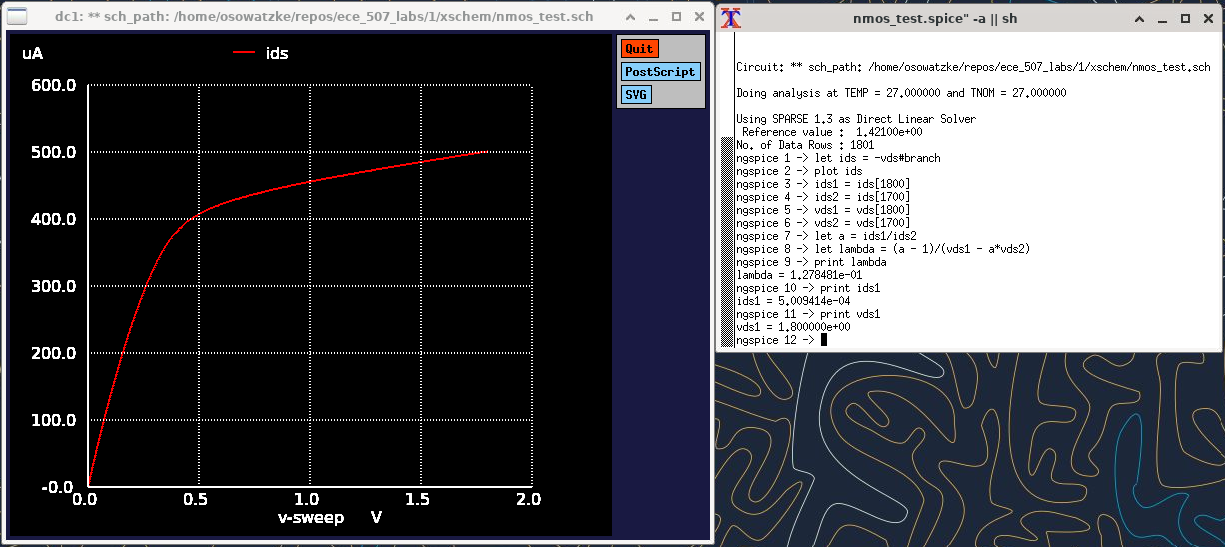
\includegraphics[width=0.8\textwidth]{nmos_lambda_meas.png}}
		\caption{NGSPICE Schematic Used to Measure the NMOS Channel Length Modulation Coefficient}
		\label{fig::nmos_lambda_meas}
	\end{figure}
	
	\noindent Using $\lambda$, we can solve for $k_n$. To do so, we use the current at $V_{ds}=1.8\ \text{V}$ and Equation \ref{eq::nmos_sat_current}. Solving for $k_n$, we obtain:
	
	\begin{equation}
		k_n = I_{ds}\left[\frac{W_n}{L}\left(V_{gs} - V_{t_n} - \frac{V_{DSAT_n}}{2}\right)V_{DSAT_n}(1 + {\lambda}V_{ds})\right]^{-1} = 321.6 {\mu}A/V^2
	\end{equation}
	
	Finally, we can solve for the body effect coefficient, $\gamma$. To do so, we compute the threshold voltage with a non-zero source-to-body voltage, $V_{SB}$. Our test circuit for this measurement is shown in Figure \ref{fig::nmos_gamma_meas_schem}.
	
	 \begin{figure}[H]
		\centerline{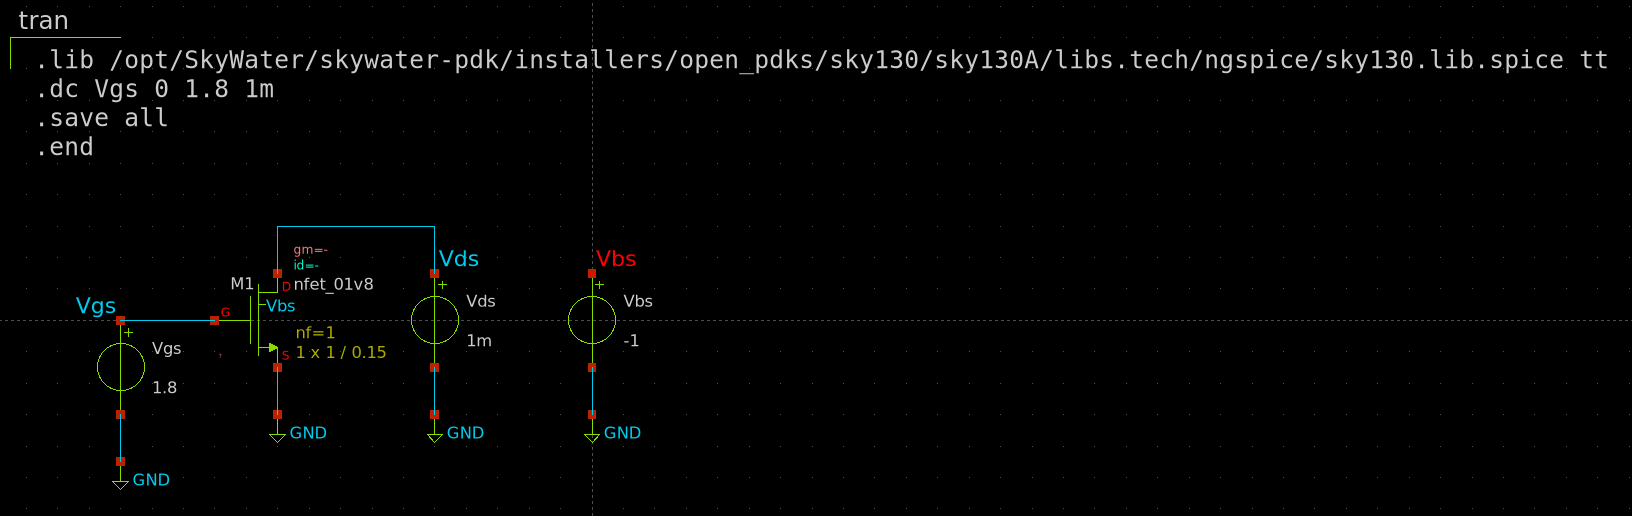
\includegraphics[width=0.8\textwidth]{nmos_gamma_meas_schem.png}}
		\caption{NGSPICE Schematic Used to Measure the NMOS Body Effect Coefficient}
		\label{fig::nmos_gamma_meas_schem}
	\end{figure}
	
	\noindent Using the test circuit, we can measure an updated threshold voltage as follows:
	
	\begin{figure}[H]
		\centerline{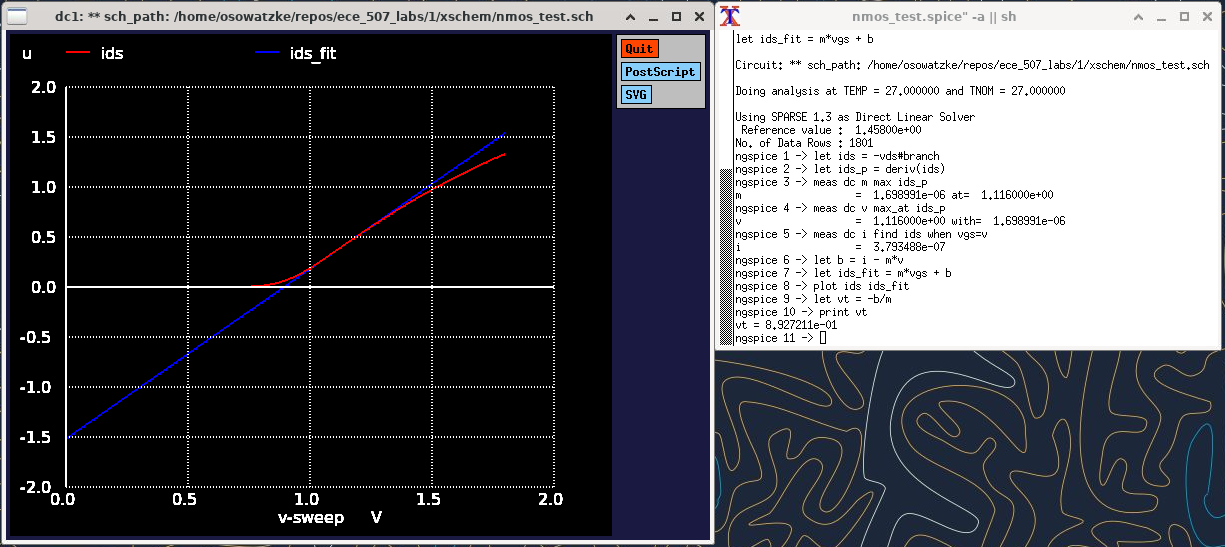
\includegraphics[width=0.8\textwidth]{nmos_gamma_meas.png}}
		\caption{Determine Updated NMOS Threshold Voltage}
		\label{fig::nmos_gamma_meas}
	\end{figure}
	
	\noindent Examining our measured data, we find that $V_T = 0.893 text{V}$. Next, we can solve for the body effect coefficient as follows:
	
	\begin{equation}
		\gamma = \frac{V_T - V_{T_0}}{\sqrt{|-2\phi_F + V_{SB}|} - {\sqrt{|-2\phi_F|}}} 
	\end{equation}
	
	\noindent Assuming $2\phi = -0.6 V$, we find that $\gamma = 0.273 V^{1/2}$. We summarize our results in Table \ref{table::nmos_derived_params} and show a fit of the data in Figure \ref{fig::nmos_iv_fit}.
	
	\begin{table}[H]
	\begin{center}
	\caption{Derived Parameters for NMOS Gate}
	\label{table::nmos_derived_params}
	\begin{tabular}{| c | c |}
		\hline
		\texttt{Parameter} & \texttt{Value}\\
		\hline	
		$V_{T_0}$ & $0.759\ \text{V}$ \\
		\hline	
		$V_{DSAT}$ & $0.202\ \text{V}$ \\
		\hline	
		$\lambda$ & $0.128\ \text{V}^{-1}$\\
		\hline	
		$k_n$ & $321.6\ {\mu}A/V^2$\\
		\hline	
		$\gamma$ & $0.273\ \text{V}^{1/2}$\\
		\hline
	\end{tabular}
	\end{center}
	\end{table}
	
	\begin{figure}[H]
		\centerline{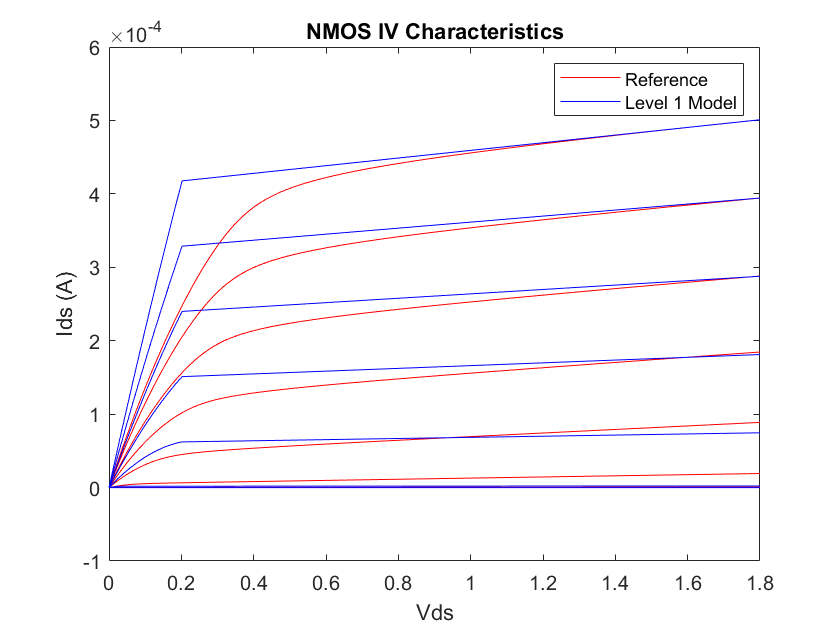
\includegraphics[width=0.8\textwidth]{nmos_iv_fit.png}}
		\caption{Fitting Level 1 Mosfet Model to NMOS IV Data}
		\label{fig::nmos_iv_fit}
	\end{figure}	
	
	\pagebreak
	\section{PMOS IV Characteristics}
	\label{appendix::pmos_iv_characteristics}
	
	In this appendix, we fit a first-order mosfet model to PMOS IV characteristics measured with the sky130A PDK. This enables us to use the equations presented in class to perform first-order analysis of our CMOS gate. We start by estimating the threshold voltage of the PMOS transistor. To perform this measurement, we use the linear extrapolation (or maximum gm) method given in \cite{cmos_vlsi_design}. Our ngspice flowchart for this analysis is given in Figure \ref{fig::pmos_vt_meas_schem}.
	
	\begin{figure}[H]
		\centerline{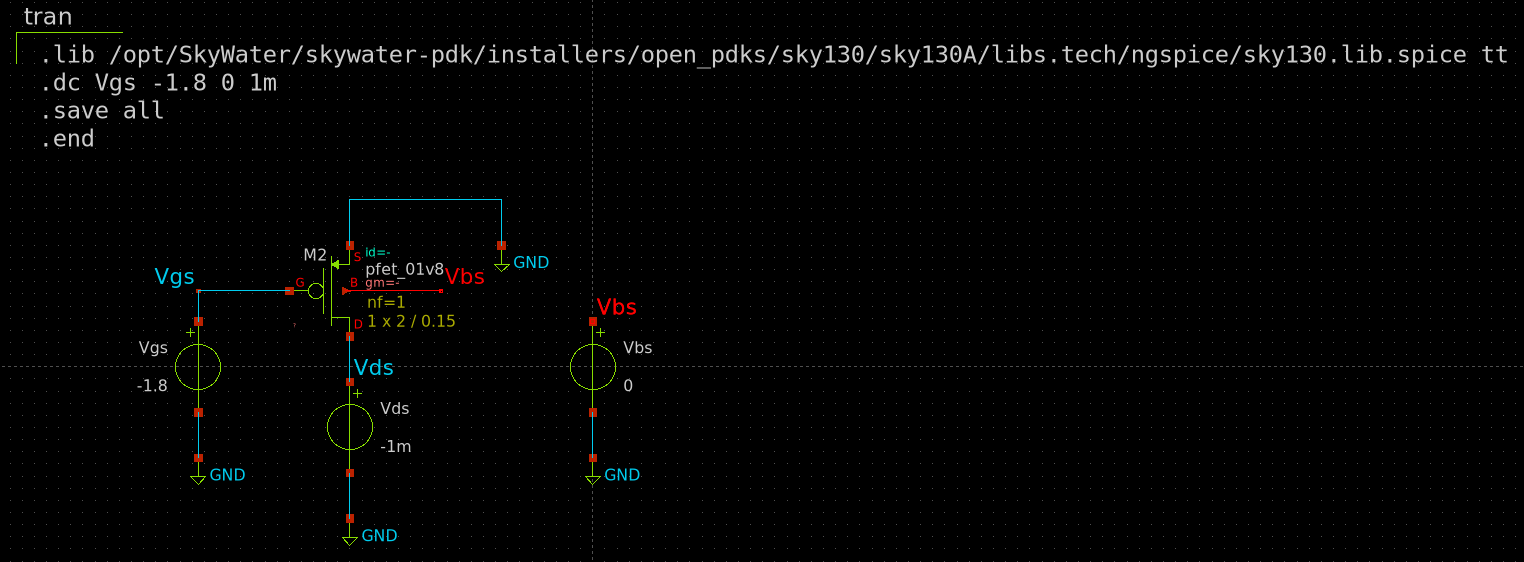
\includegraphics[width=0.8\textwidth]{pmos_vt_meas_schem.png}}
		\caption{NGSPICE Schematic Used to Measure the PMOS Threshold Voltage}
		\label{fig::pmos_vt_meas_schem}
	\end{figure}
	
	\noindent Using the flowchart, we examine the drain current for the PMOS transistor in the linear region of operation. In this region, the drain current of the PMOS transistor is given as follows:
	
	\begin{equation}
		I_{ds} = k_p\frac{W_p}{L}\left(V_{gs} - V_{t_p} - \frac{V_{ds}}{2}\right)V_{ds}
	\end{equation}
	
	\noindent To fit the IV characteristics, we estimate the $I_{ds}$ curve with a line that is tangent to the point with maximum-slope. We then define $V_t$ as the voltage at which the estimated current is zero. This procedure is illustrated in Figure \ref{fig::pmos_vt_meas}, which predicts a threshold voltage of -0.793 V.
	
	\begin{figure}[H]
		\centerline{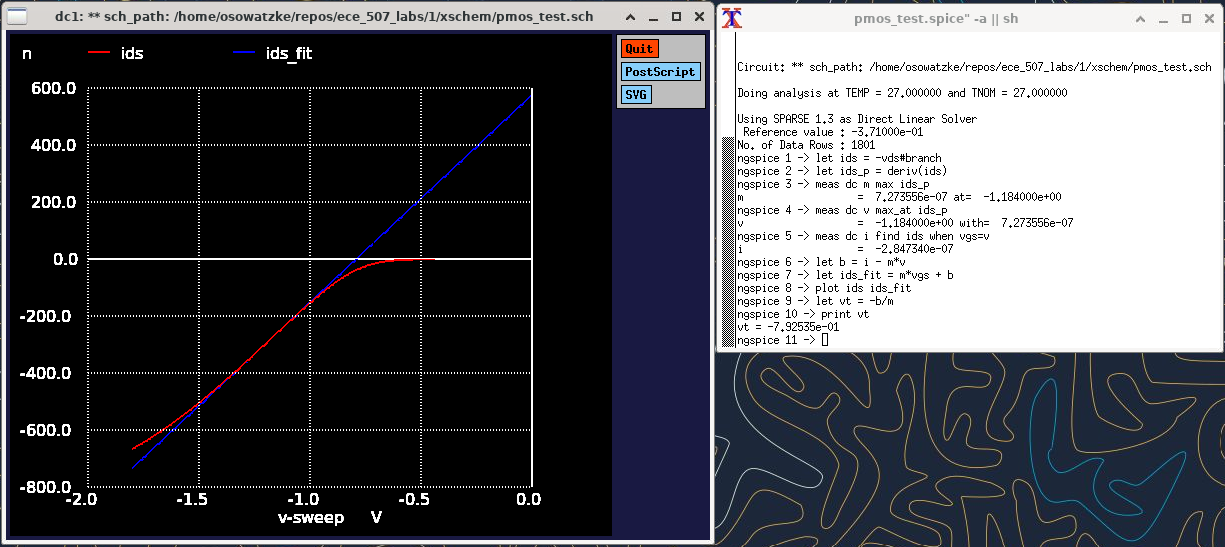
\includegraphics[width=0.8\textwidth]{pmos_vt_meas.png}}
		\caption{Estimating PMOS Threshold Voltage}
		\label{fig::pmos_vt_meas}
	\end{figure}
	
	Next, we measure the saturation voltage. We use the flowchart shown in Figure \ref{fig::pmos_vt_meas_schem} to perform this measurement.
	
	\begin{figure}[H]
		\centerline{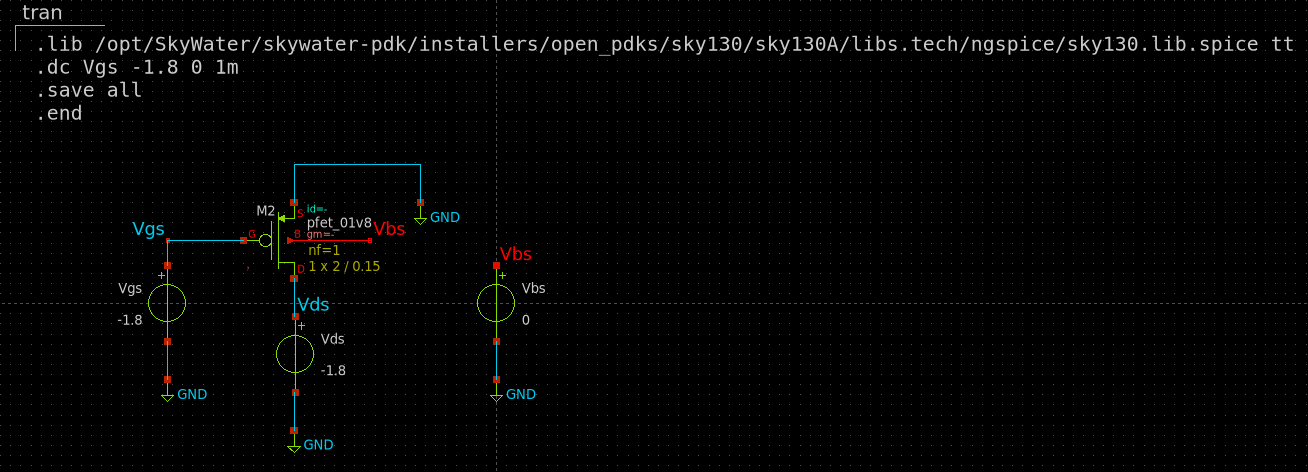
\includegraphics[width=0.8\textwidth]{pmos_vdsat_meas_schem.png}}
		\caption{NGSPICE Schematic Used to Measure the PMOS Saturation Voltage}
		\label{fig::pmos_vdsat_meas_schem}
	\end{figure}
	
	 \noindent In the above schematic, we consider the drain current in the velocity saturation region. The drain current in this region is defined as follows:
	
	\begin{equation}
		\label{eq::pmos_sat_current}
		I_{ds} = k_p\frac{W_p}{L}\left(V_{gs} - V_{t_p} - \frac{V_{DSAT_p}}{2}\right)V_{DSAT_p}(1 + {\lambda}V_{ds})
	\end{equation}
	
	\noindent If we analyze the ratio of drain currents for the same values of $V_{ds}$ and different values of $V_{gs}$, we can express the ratios as follows:
	
	\begin{equation}
		\frac{V_{gs_1} - V_{t_n} - V_{DSAT_p}/2}{V_{gs_2} - V_{t_n} - V_{DSAT_p}/2} = \frac{V_{gs_1} - V}{V_{gs_2} - V} = \frac{I_{ds_1}}{I_{ds_2}} = \alpha
	\end{equation}
	
	\noindent Solving for $V$, we obtain the following:
	
	\begin{equation}
		V = \frac{{\alpha}V_{gs_2} - V_{gs_1}}{\alpha - 1}
	\end{equation}
	
	\noindent where $V_{DSAT_p} = 2(V - V_{t_p})$. Following the procedure outlined above, we execute the following commands in ngspice to derive the saturation voltage. Our work is shown in Figure \ref{fig::pmos_vdsat_meas} and we find that $V_{DSAT_p} = -0.361\ \text{V}$.
	
	\begin{figure}[H]
		\centerline{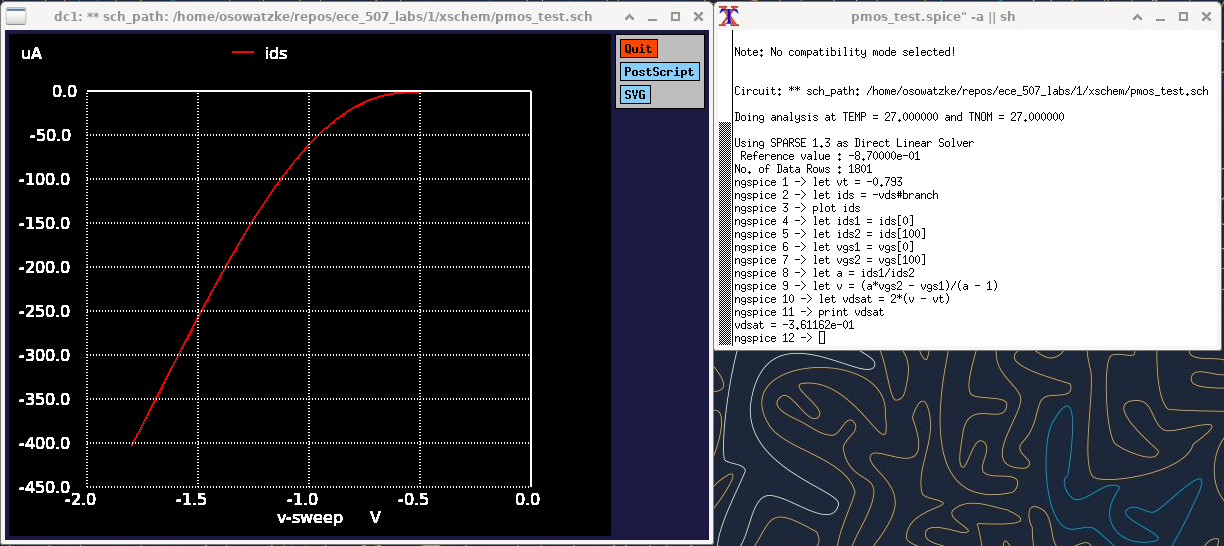
\includegraphics[width=0.8\textwidth]{pmos_vdsat_meas.png}}
		\caption{Measuring the PMOS Saturation Voltage}
		\label{fig::pmos_vdsat_meas}
	\end{figure}
	
	Then, we find the channel length modulation coefficient $\lambda$. To do this, we use the NGSPICE schematic shown in Figure \ref{fig::pmos_lambda_meas_schem}.
	
	\begin{figure}[H]
		\centerline{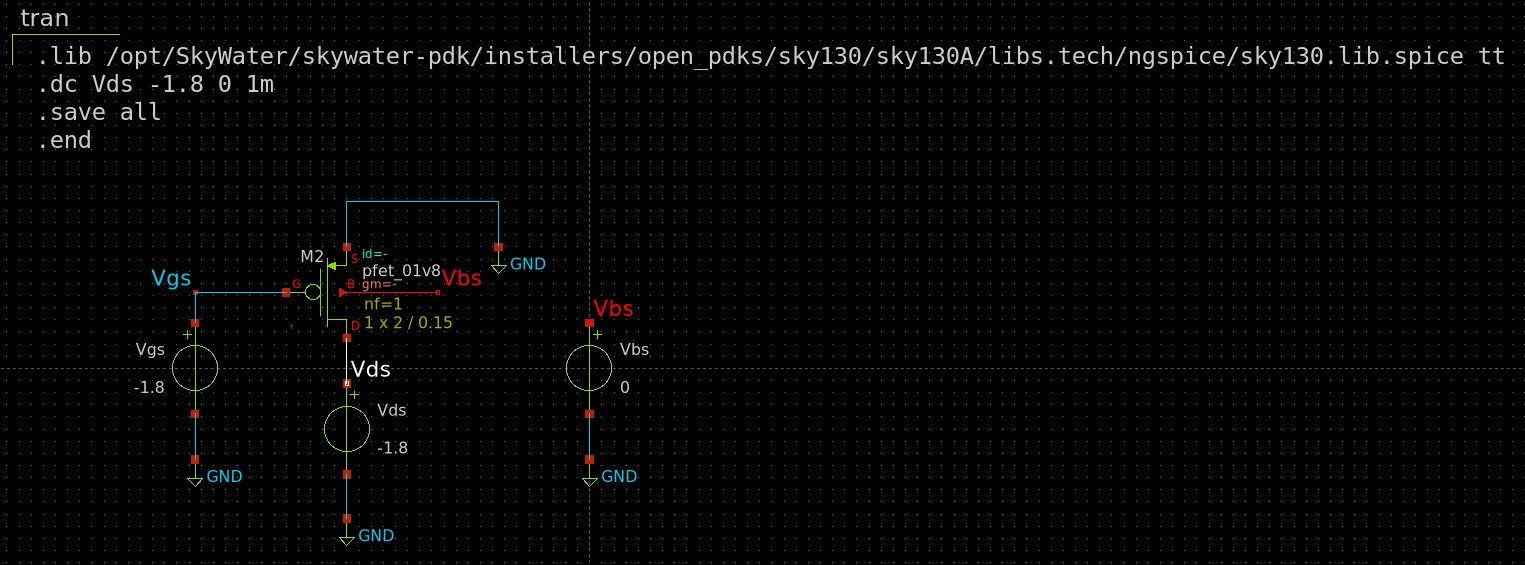
\includegraphics[width=0.8\textwidth]{pmos_lambda_meas_schem.png}}
		\caption{NGSPICE Schematic Used to Measure the PMOS Channel Length Modulation Coefficient}
		\label{fig::pmos_lambda_meas_schem}
	\end{figure}
	
	\noindent Here, we once again consider currents in the velocity saturation state. We specifically look at the ratios of currents when varying $V_{ds}$ and keeping $V_{gs}$ constant. Doing so, we obtain the following:
	
	\begin{equation}
		\frac{1 + {\lambda}V_{ds_1}}{1 + {\lambda}V_{ds_2}} = \frac{I_{ds_1}}{I_{ds_2}} = \alpha
	\end{equation}
	
	\noindent Solving for $\lambda$, we obtain the following:
	
	\begin{equation}
		\lambda = \frac{\alpha - 1}{V_{ds_1} - V_{ds_2}}
	\end{equation}
	
	\noindent In Figure \ref{fig::pmos_lambda_meas}, we perform this analysis for the PMOS circuit and find that $\lambda = -0.335 V^{-1}$.
	
	\begin{figure}[H]
		\centerline{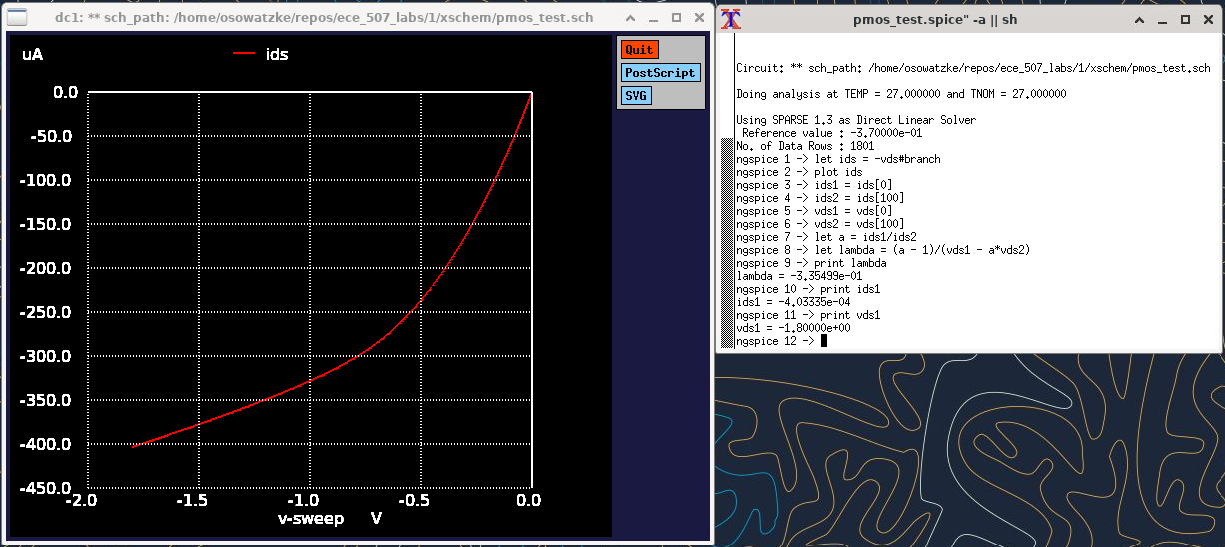
\includegraphics[width=0.8\textwidth]{pmos_lambda_meas.png}}
		\caption{NGSPICE Schematic Used to Measure the PMOS Channel Length Modulation Coefficient}
		\label{fig::pmos_lambda_meas}
	\end{figure}
	
	\noindent Using $\lambda$, we can solve for $k_p$. To do so, we use the current at $V_{ds}=-1.8\ \text{V}$ and Equation \ref{eq::pmos_sat_current}. Solving for $k_p$, we obtain:
	
	\begin{equation}
		k_p = I_{ds}\left[\frac{W_p}{L}\left(V_{gs} - V_{t_p} - \frac{V_{DSAT_p}}{2}\right)V_{DSAT_p}(1 + {\lambda}V_{ds})\right]^{-1} = -63.25 {\mu}A/V^2
	\end{equation}
	
	Finally, we can solve for the body effect coefficient, $\gamma$. To do so, we compute the threshold voltage with a non-zero source-to-body voltage, $V_{SB}$. Our test circuit for this measurement is shown in Figure \ref{fig::pmos_gamma_meas_schem}.
	
	 \begin{figure}[H]
		\centerline{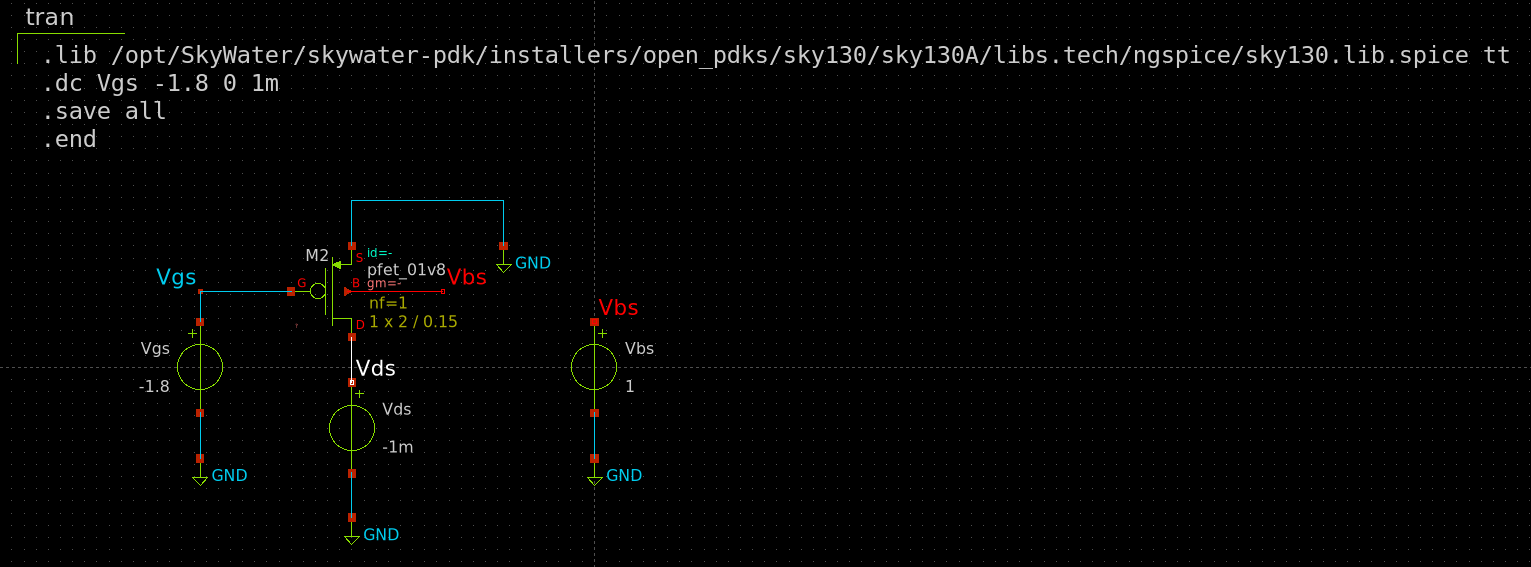
\includegraphics[width=0.8\textwidth]{pmos_gamma_meas_schem.png}}
		\caption{NGSPICE Schematic Used to Measure the PMOS Body Effect Coefficient}
		\label{fig::pmos_gamma_meas_schem}
	\end{figure}
	
	\noindent Using the test circuit, we can measure an updated threshold voltage as follows:
	
	\begin{figure}[H]
		\centerline{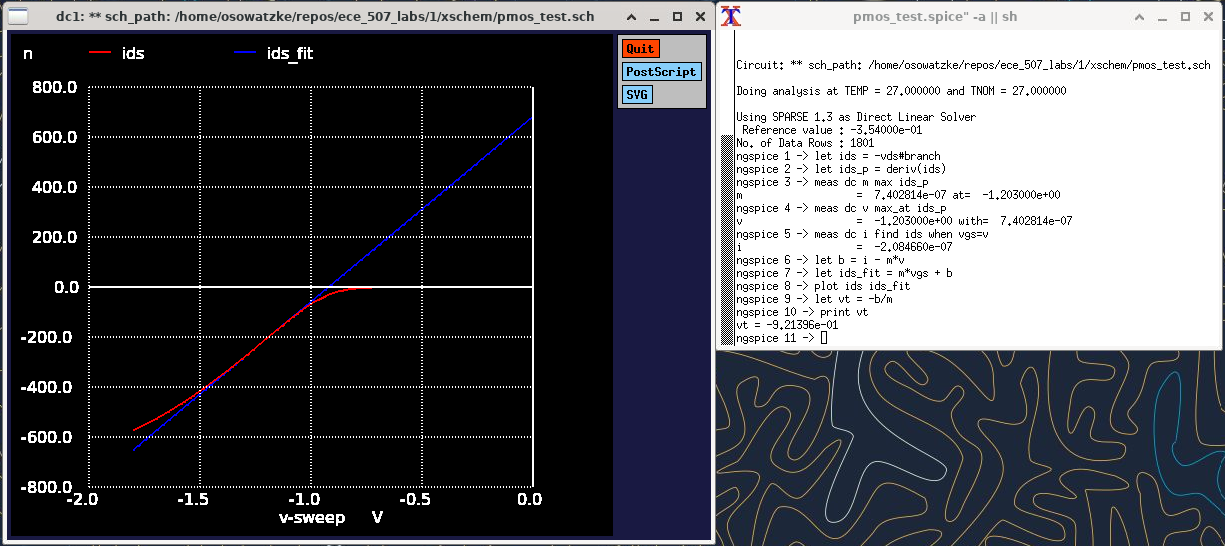
\includegraphics[width=0.8\textwidth]{pmos_gamma_meas.png}}
		\caption{Determine Updated PMOS Threshold Voltage}
		\label{fig::pmos_gamma_meas}
	\end{figure}
	
	\noindent Examining our measured data, we find that $V_T = -0.921\ \text{V}$. Next, we can solve for the body effect coefficient as follows:
	
	\begin{equation}
		\gamma = \frac{V_T - V_{T_0}}{\sqrt{|-2\phi_F - V_{SB}|} - {\sqrt{|-2\phi_F|}}} 
	\end{equation}
	
	\noindent Assuming $2\phi = -0.6 V$, we find that $\gamma = -0.261 V^{1/2}$. We summarize our results in Table \ref{table::pmos_derived_params} and show a fit of the data in Figure \ref{fig::pmos_iv_fit}.
	
	\begin{table}[H]
	\begin{center}
	\caption{Derived Parameters for PMOS Gate}
	\label{table::pmos_derived_params}
	\begin{tabular}{| c | c |}
		\hline
		\texttt{Parameter} & \texttt{Value}\\
		\hline	
		$V_{T_0}$ & $-0.793\ \text{V}$ \\
		\hline	
		$V_{DSAT}$ & $-0.361\ \text{V}$ \\
		\hline	
		$\lambda$ & $-0.335\ \text{V}^{-1}$\\
		\hline	
		$k_p$ & $-63.25\ {\mu}A/V^2$\\
		\hline	
		$\gamma$ & $-0.261\ \text{V}^{1/2}$\\
		\hline
	\end{tabular}
	\end{center}
	\end{table}
	
	\begin{figure}[H]
		\centerline{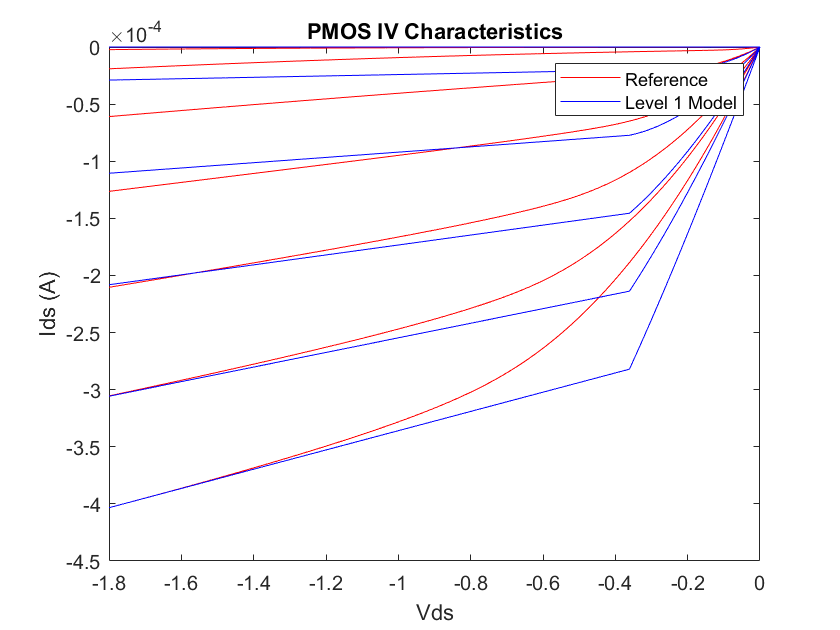
\includegraphics[width=0.8\textwidth]{pmos_iv_fit.png}}
		\caption{Fitting Level 1 Mosfet Model to PMOS IV Data}
		\label{fig::pmos_iv_fit}
	\end{figure}

\end{document}